\chapter{Experiments}\label{chapter:experiments}

\section{Experimental Setup}
We use the openTSNE library \textcolor{red}{which version?} for all of our experiments. Unless otherwise specified, we always use the default openTSNE settings \comment{describe them here}. 

We want to perform our experiments on a variety of different datasets, from typically used benchmark datasets, Macosko and MNIST, to very small (Iris) and very large datasets (Flow18). We use the following in our experiments: 
\begin{itemize}
    \item \textbf{Iris} flower dataset \cite{iris_dataset}. This small dataset contains 50 samples from three different species of Iris flowers, thus 150 points in total. Datapoints are comprised of four features, namely the length and width of sepals and petals. 
    \item \textbf{Macosko} mouse retina cells dataset\cite{Macosko_dataset}. This is common benchmark dataset for single-cell data. It contains a total of 44,808 datapoints. The features are given by the high-dimensional gene-expression profiles outlined in \cite{Macosko_dataset}. 
    Here, we also apply PCA to reduce the dimensionality of the dataset to 50 before performing t-SNE. 
    \comment{\cite{KoBe19SingleCell} say this has 39 classes but I thought we only looked at 12?}
    \item \textbf{MNIST} \cite{mnist_dataset}: A classic computer vision dataset, contains $N=70,000$ gray scale images of handwritten digits 0 throuh 9 (i.e. 10 classes). 
    Each image has dimensionality $D=28 \cdot 28 = 784$. Before applying t-SNE, we rescale the entries to values in the interval $[0,1]$ and reduce the dimensionality of data points to 50 using PCA.  
    \item \textbf{Flow18} cytometry dataset \cite{flow_dataset}. 
    One millon datapoints, samples are human PBMC (peripheral blood mononuclear cells), so for example different types of T cells, white blood cells or B cells. 
    The dataset consists of 16 (\textcolor{red}{only 15 if dead and lin- considered together}) different classes of cells. For each cell, 18 parameters are recorded of which we use 11 for our visualization, just as in \cite{belkina19}. 
    \textcolor{red}{TODO: look up how many samples there are per class, also: maybe run experiments again with dead cells and Lin- cells in the same class}
\end{itemize}
\section{Quality Evaluation Metrics}
Measuring the quality of t-SNE embeddings is challenging. 
Of course, since the point of t-SNE is primarily visualization, we will look at the scatterplots the algorithm produces first and foremost. 

However, we will also use several other quality evaluation metrics in order to get a broader understanding of the quality of our results. 
\begin{itemize}
    \item \textbf{KLD}: like \cite{belkina19}, we measure Kullback Leibler divergence throughout the algorithm and compare endpoint KLD values, the smaller the better. 
    It should be noted that KLD is not a good measure when comparing t-SNE embeddings with different perplexity values since this directly affects KLD. 
    The same is true to some extent for early exaggeration.  
    \item \textbf{KNN}: for every data point, we measure the fraction of $k$-nearest neighbors in the high-di\-mension\-al space that are preserved as $k$-nearest neighbors in the low-di\-men\-sio\-nal embedding space, see \cite{KoBe19SingleCell}. 
    We use the code from \comment{insert github of kobak et. al}. 
    This measures local structure. 
    We set $k=10$. 
    \item \textbf{KNC}: this measures the percentage of $k$-nearest class means preserved in the low-dimensional embedding, averaged across all classes. (\comment{von jime: man schaut sich mittelpunkt von den klassen an und alle anderen naechsten mittelpunkte und dann schaut man wie viele davon perserved werden})
    We use $k=3$ (\comment{check this, cite BA statistik}). 
    This \enquote{quantifies perservation of the mesoscopic structure} \cite{KoBe19SingleCell}. 
    \item \textbf{CPD}: We calculate the Spearman correlation between high and low-dimensional distances across 1000 randomly chosen pairs of distances. This is repeated 10 times, we take the averaged result, as suggested by \comment{cite BA}. This is a measure to quantify the global structure of our data. \comment{TODO: Insert formula fpr CPD}
\end{itemize}


\section{Dataset Cluster Assumptions}
Here we investigate if assumptions made for clustering results in \cite{LinStei22} hold in practice, by looking at the simple Iris dataset. 
The reason that we look at Iris is that it is a very small dataset, which makes it feasible to look at all $N^2 = 150^2$ affinities $p_{ij}$ individually.  

Recalling \ref{eq:4.1}, we make the assumption that the data we perform t-SNE on is clustered. 
A natural question to ask then is: does real-life data that looks clustered to us humans fulfill this definition of clustered that is required: 
\begin{equation}
    p_{ij} \geq \frac{1}{10 N |\Omega(i)|}
\end{equation}
for all pairs of points $x_i, x_j$ that lie in the same cluster $\Omega(i)$? 

In order to investigate this question, we chose the Iris dataset. 
Ordering the data points in terms of cluster membership (there are 50 points of each of the three clusters), we can visualize what the high-dimensional similarity values $p_{ij}$ look like when using the standard parameters (perplexity = 30). 

\begin{figure}[h]
    %\begin{center}
    \centering 
        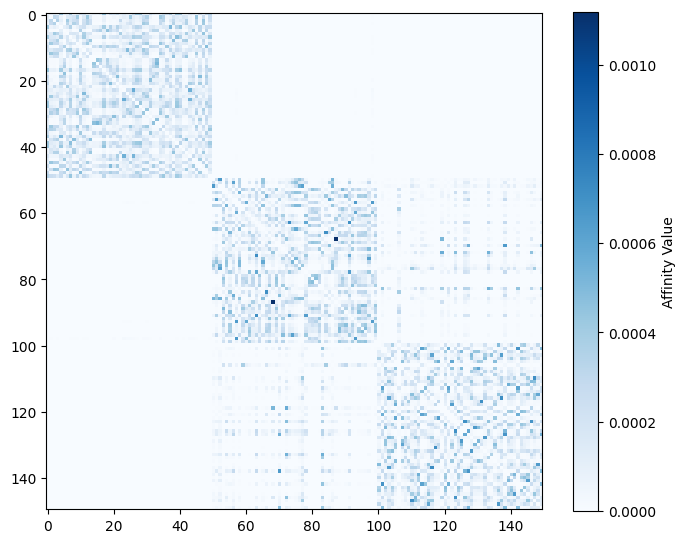
\includegraphics[width=0.7\linewidth]{figures/iris_affinity_matrix.png}
        \caption{Affinity values $p_{ij}$ of the Iris dataset visualized. The affinity matrix was generated using the standard perplexity value of 30.}
    %\end{center}
    \label{fig:iris_affinities}
\end{figure}

We can see the three clusters of the Iris dataset pretty clearly. 
From the visualization \ref{fig:iris_affinities}, it also seems like the first cluster is more well-defined than the second and third are. 
\textcolor{red}{If we run a dimensionality algorithm like PCA or t-SNE on it, we can also see that it performs well and clearly separates at least the first cluster from the other two.} 

So, it would seem that at least this first cluster would fulfil the condition that \begin{equation} p_{ij} \geq \frac{1}{10 N |\Omega(i)|} = \frac{1}{10 \cdot 150 \cdot 50} \end{equation}

However, when we investigate the $p_{ij}$ values of the first cluster (excluding, of course, the diagonal elements, since they are always zero), we notice that the smallest $p_{ij}$ value we observe is (rounded) $2.8 \cdot 10^{-7}$, whereas we calculated a lower bound of about $1.3 \cdot 10^{-5}$ above.
Furthermore, we calculated that a total number of 354 similarites between points in this same first cluster are smaller than the minimal $p_{ij}$ value required for it to be a cluster. 
Now, while \cite{LinStei22} do mention that there is some flexibility with respect to the exact constant being used - we would have to increase it by two orders of magnitude for this result to hold. 

For the last two clusters, we observe something even more interesting. 
If we consider the second cluster, we see that that the smallest similarity value between two points in it is $0.0$. 
This makes it virtually impossible to consider as a cluster, not matter how far we would scale the constant. 
One might argue that indeed clusters 2 and 3 belong together, but also then we observe some points having $0$ similarity to each other. 

\section{Initialization}
As mentioned above, the benefits of PCA initialization are well-studied (\textcolor{red}{include references here}). 
For example, \cite{kobak21} showed that t-SNE is better able to recover a synthetic 2D circle when initialized with PCA. 

Building on this work \textcolor{red}{and using their code (maybe I should cite the github here)}, we show that t-SNE also recovers other geometric structures like triangles (\ref{fig:triangle}) and squares (\ref{fig:square}) better when initialized with PCA. 

Implementation details: we sampled $n=7000$ points and added some Gaussian noise. We closely followed \cite{kobak21}, only changing the circle to a triangle and square. 

We also use two different seeds for each of the embeddings with random and PCA initialization. 
As expected, we see much more variance in the embedding when we use random initialization. While using PCA initialization eliminates some of this variance between embeddings, we can still observe small differences between the embeddings (especially of the triangle). 

\begin{figure}[h]
    \centering 
        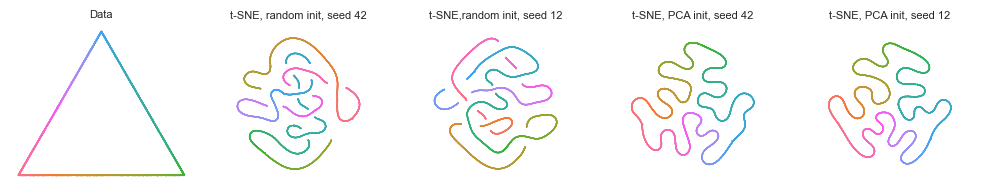
\includegraphics[width=\linewidth]{figures/t_sne_on_triangle.png}
        \caption{t-SNE on an equilateral triangle in 2D space. Using PCA initialization improves recovery of the structure better than when using random initialization.}
    \label{fig:triangle}
\end{figure}

\begin{figure}[h]
    \centering 
        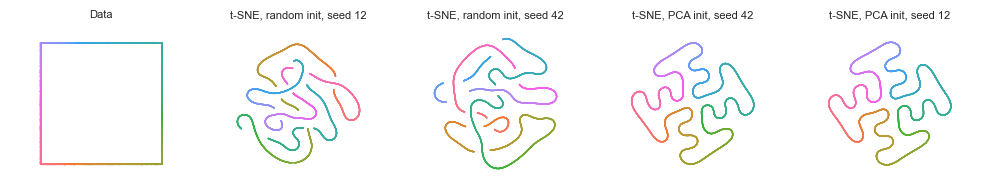
\includegraphics[width=\linewidth]{figures/t_sne_on_square.png}
        \caption{t-SNE performed on a square (with some Gaussian noise added) \textcolor{red}{the seeds of the first two embeddings here are switched up, it should be seed 42 first}}
    \label{fig:square}
\end{figure}

We thought it was interesting to see how PCA initialization helps with preserving geometric structures and to see that PCA-initialized t-SNE embeddings with different seeds still lead to slightly different results. 
But ultimately, it is well-established in the research that PCA should be used to initilize the low-dimensional embedding. 
We will therefore not conduct any other experiments regarding initialization. 

\textcolor{red}{TODO: think about if I want to say something about spectral initialization}

\section{Number of Iterations}
We ran t-SNE with a different number of iterations on the 4 datasets above. Our expectation was that bigger datasets need more iterations. The EE length was kept at 25 percent of the total number of iterations. 

\begin{figure}[h]
    \centering 
        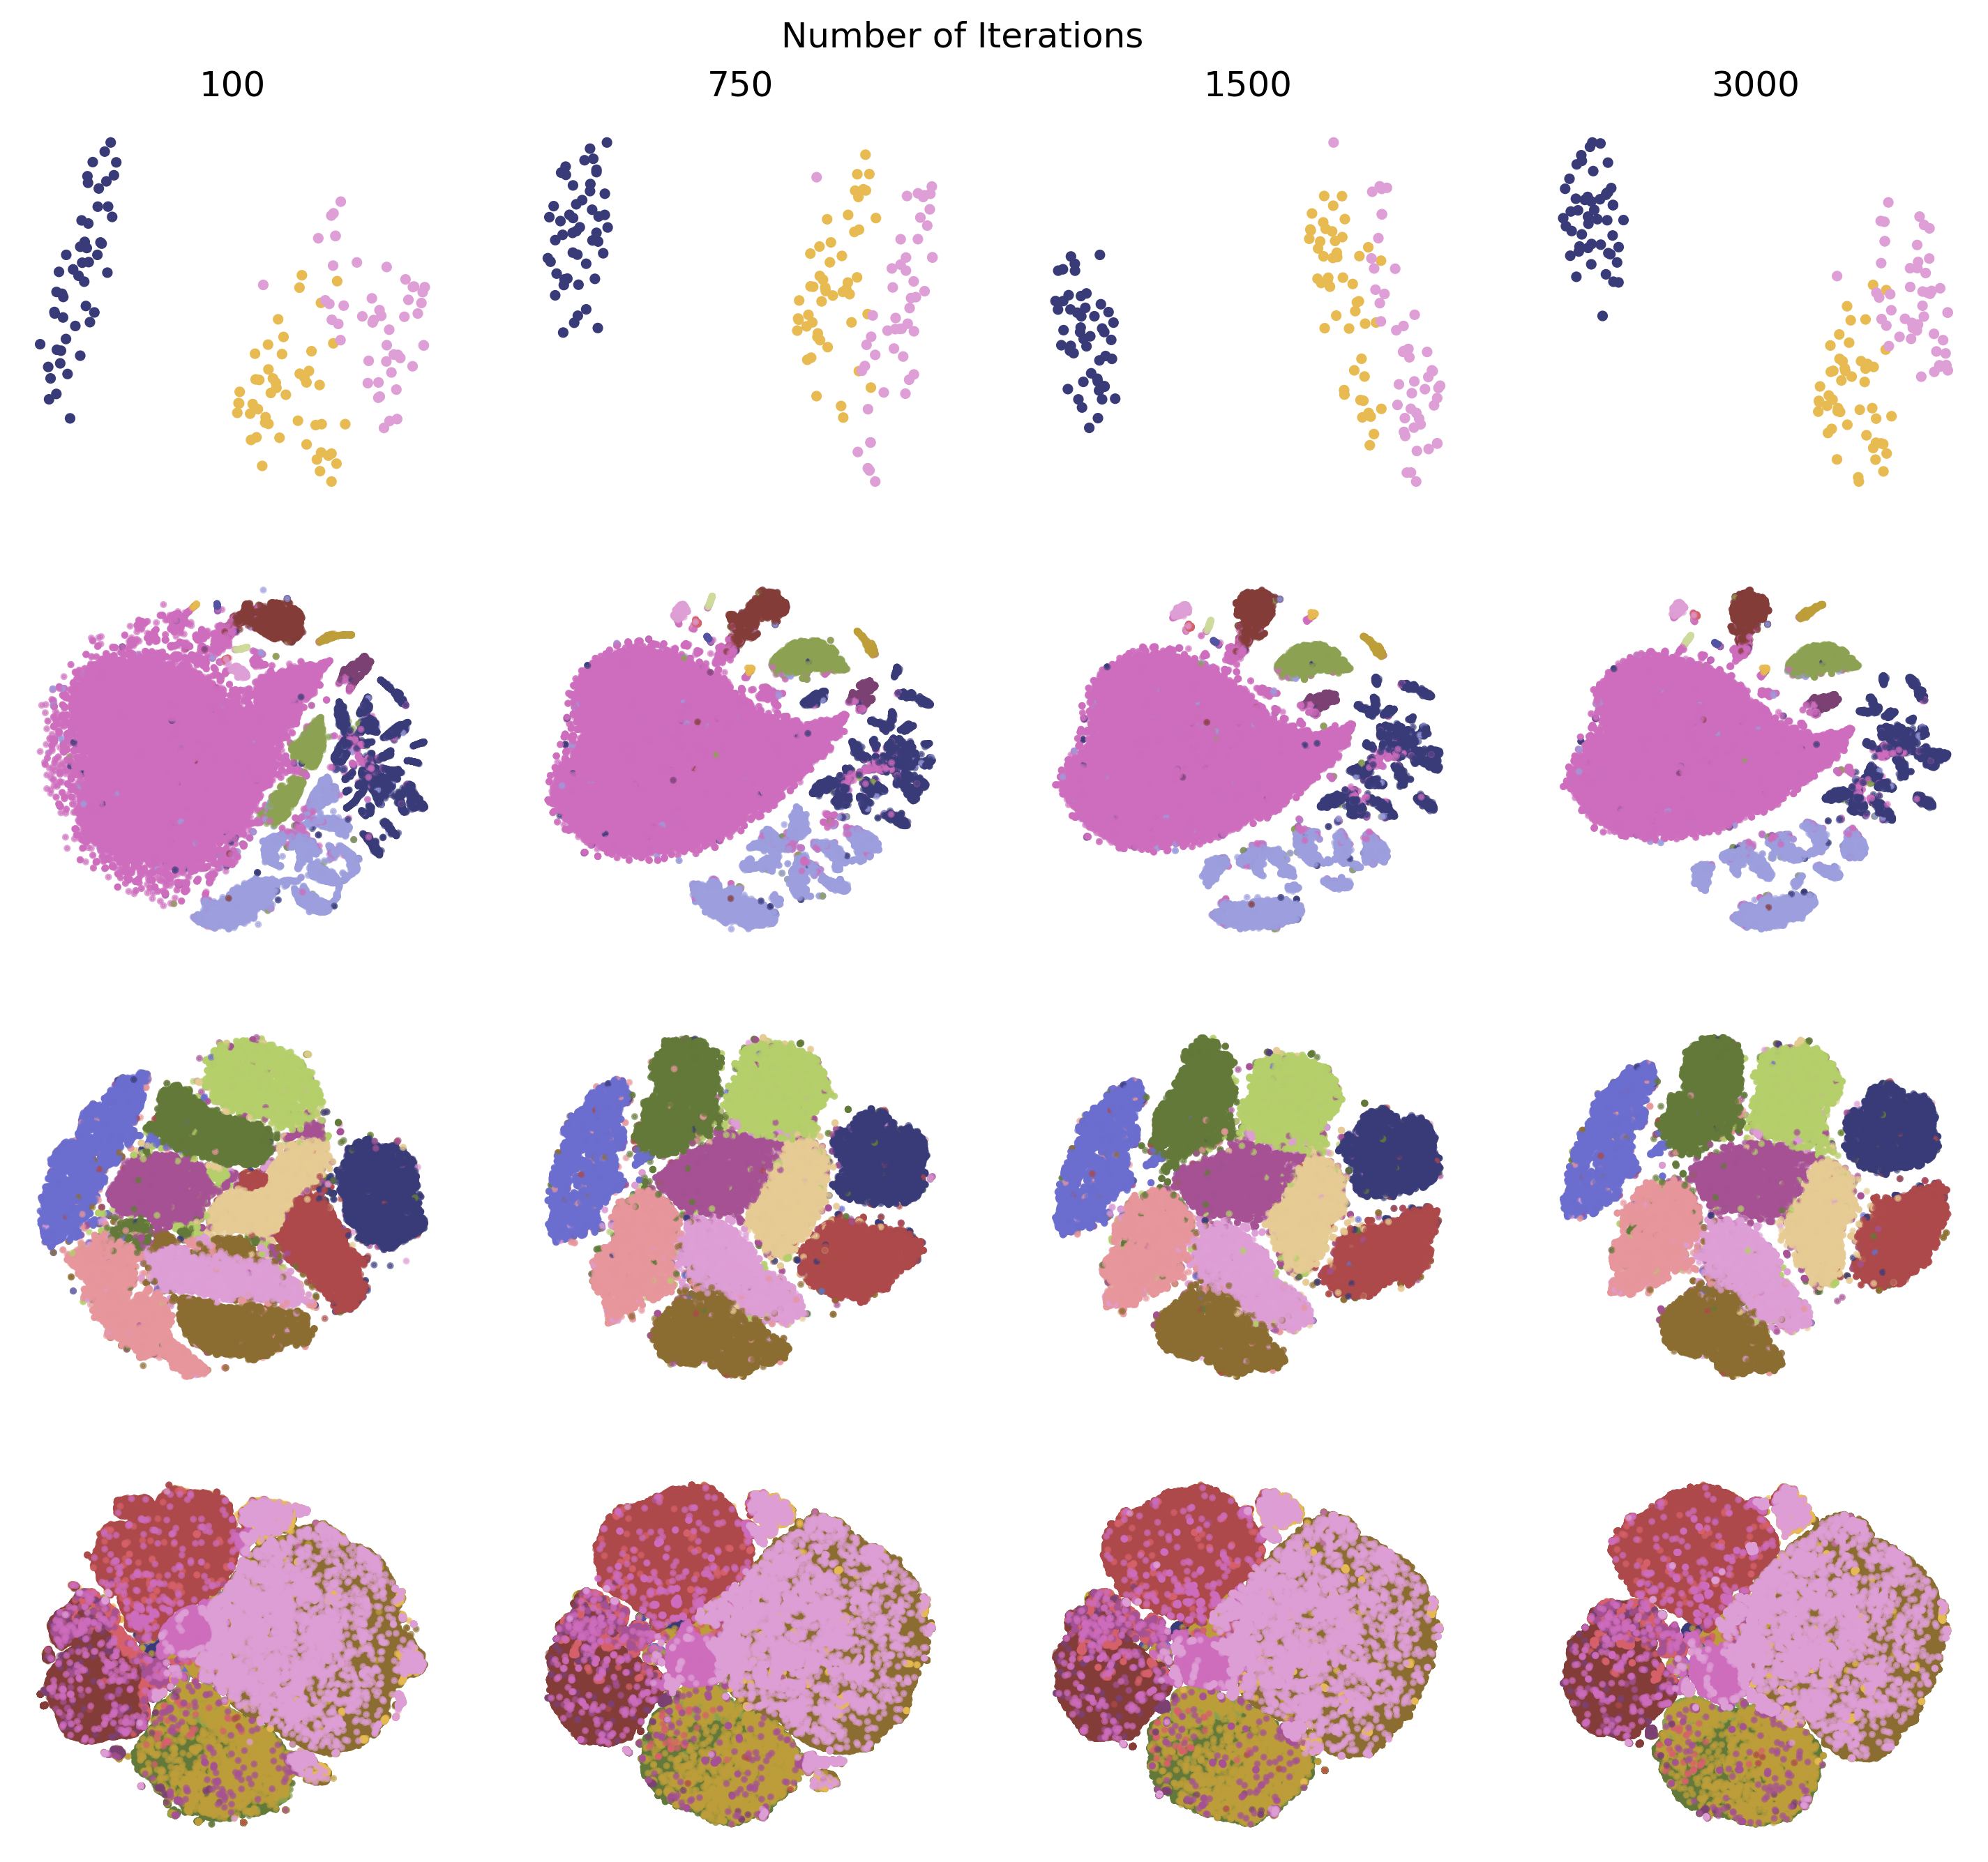
\includegraphics[width=\linewidth]{figures/n_iter/n_iter_embedding_grid_tab20b.png}
        \caption{Embeddings of the four datasets.}
    \label{fig:n_iter-grid}
\end{figure}

\begin{figure}[h]
    \centering 
        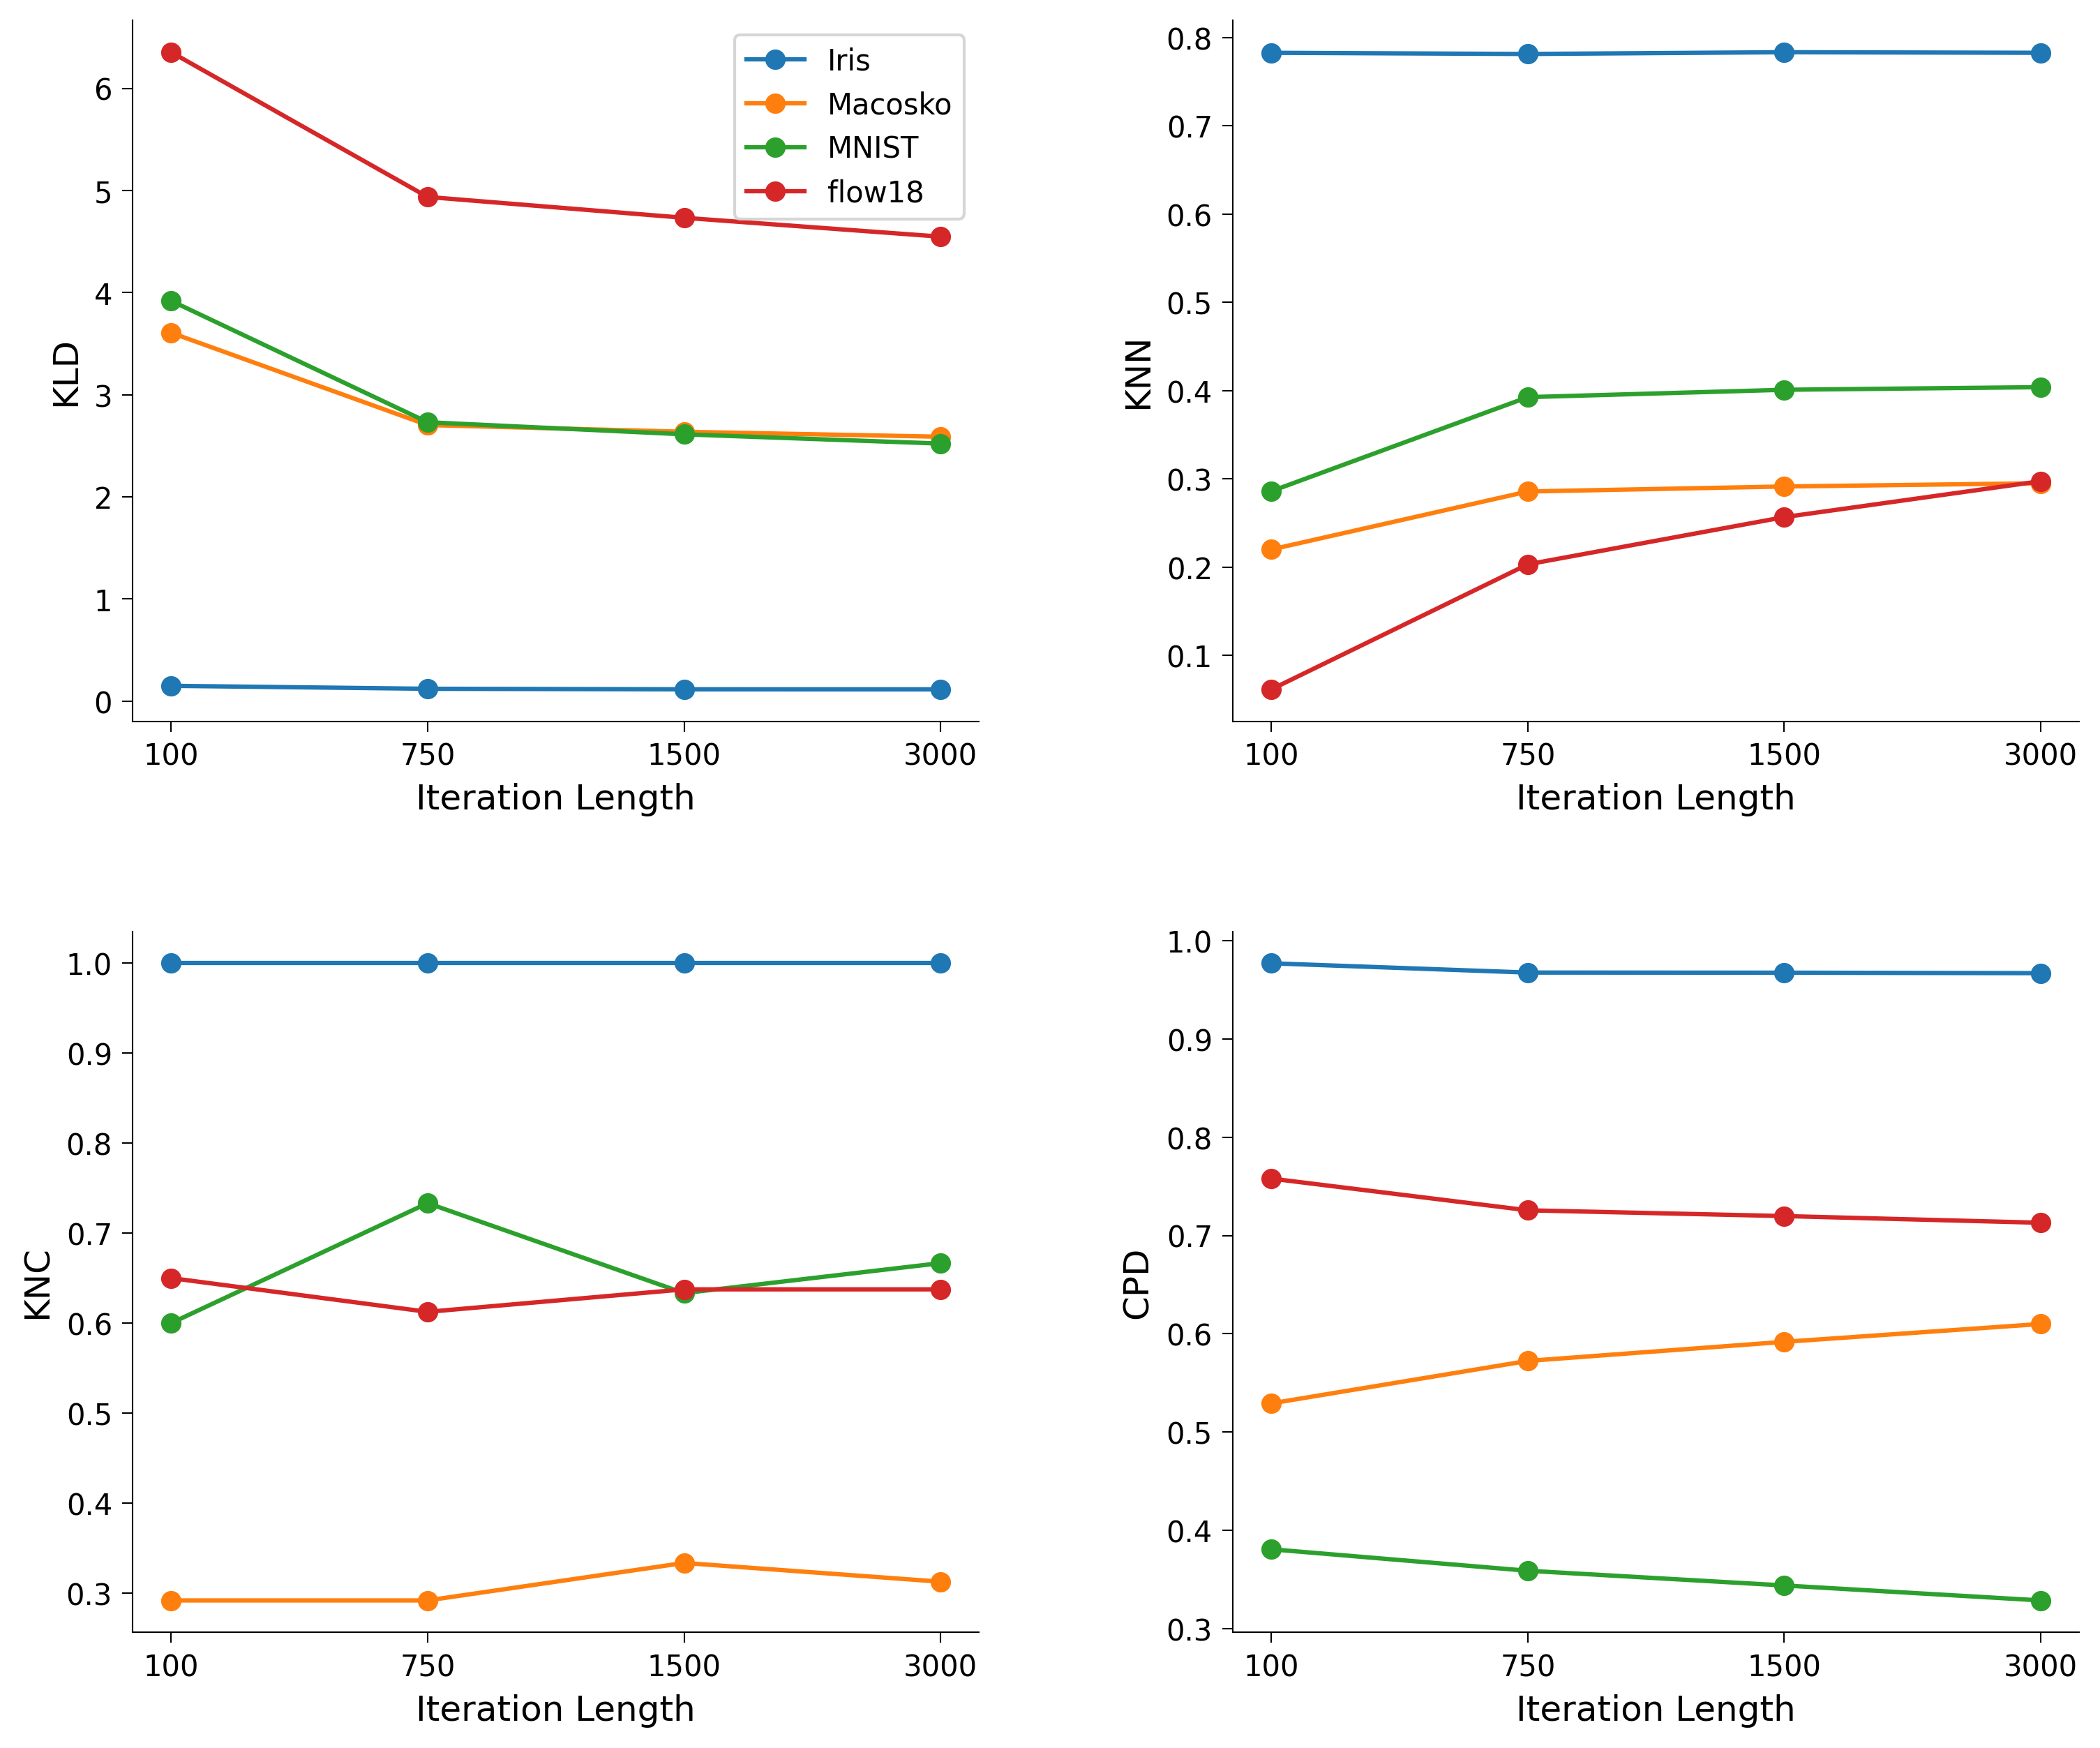
\includegraphics[width=\linewidth]{figures/n_iter/n_iter_4_quality_measures.png}
        \caption{quality measures. say what they show here.}
    \label{fig:n_iter-quality}
\end{figure}

We can observe that even 100 iterations is enough on the small Iris dataset. 
With 100 iterations, the embedding took 0.55 seconds to run, whereas the standard number of 750 iterations took 2.42 seconds. 
We also see that the largest dataset, Flow18, profits the most from the largest number of iterations, as expected. 

\newpage 
\section{An Implementation of Rescaled t-SNE for Large Data Limits}
For the Gaussian mixture data, we use $b=0.03$ and for MNIST $b=0.07$. In both cases $\kappa=15$ is used. 

\begin{figure}[h]
    \centering 
        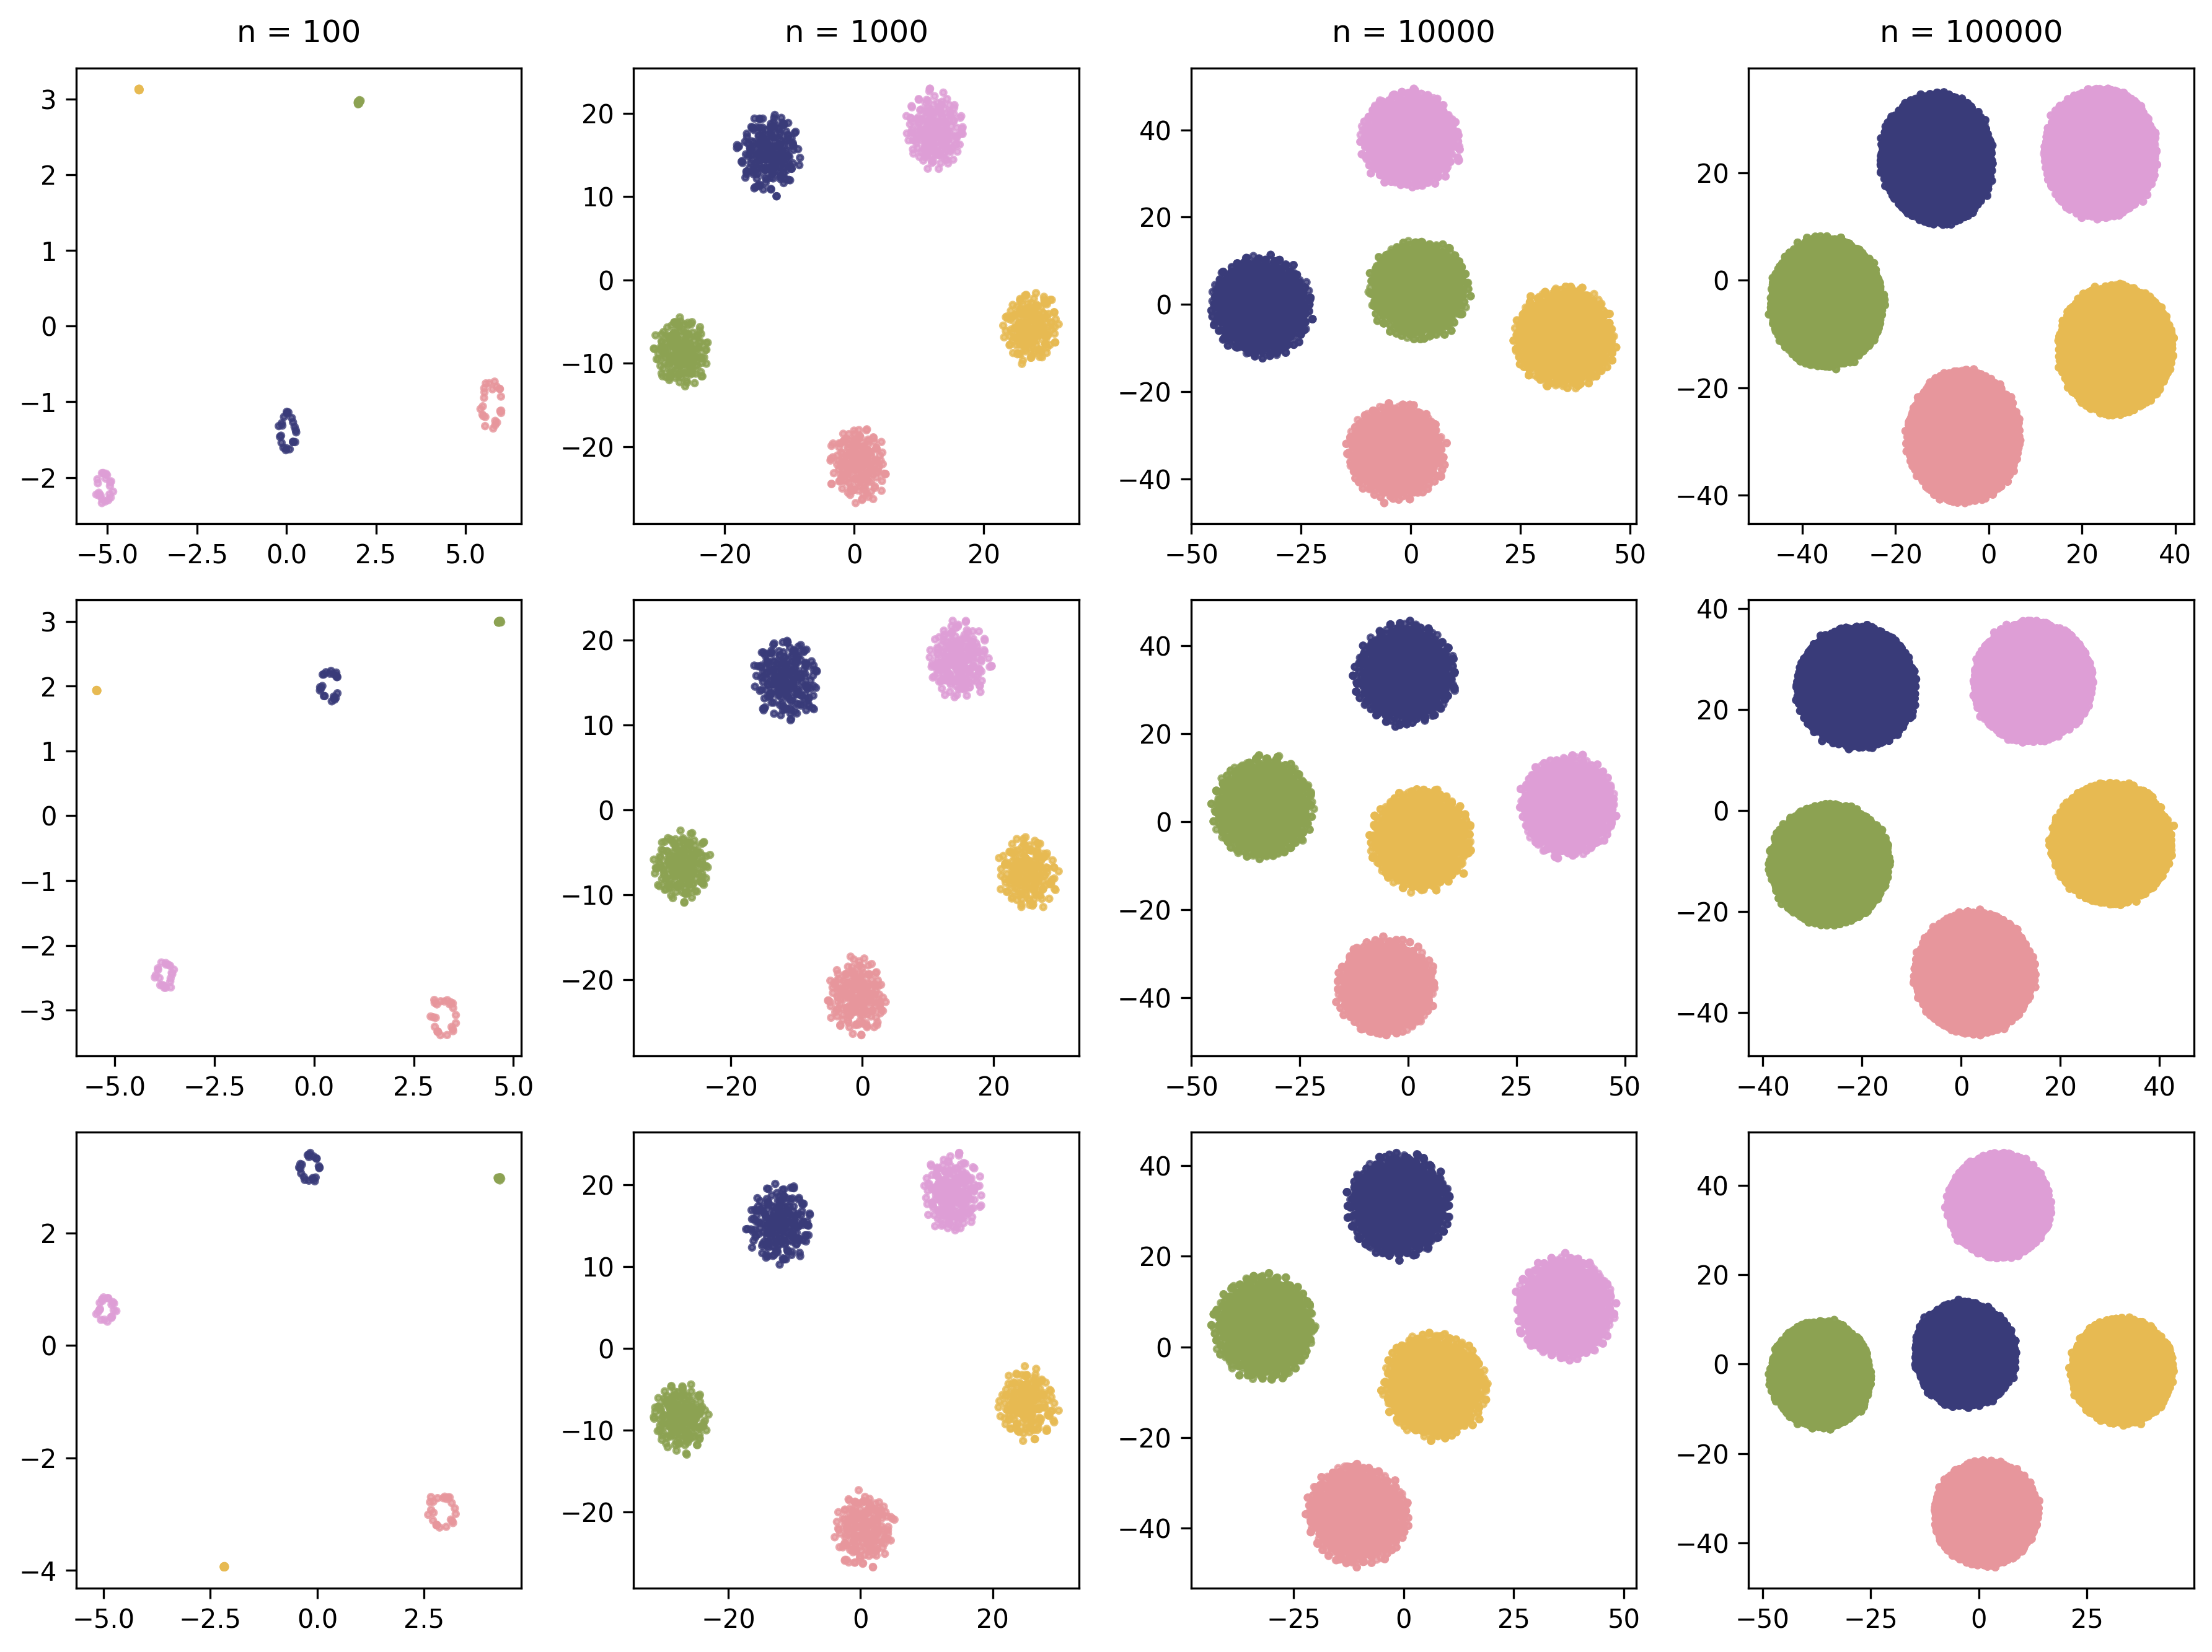
\includegraphics[width=\linewidth]{figures/rescaled/Gaussian_Mixture_standard_embedding_grid.png}
        \caption{Using standard t-SNE. Data generated from mixture of five Gaussian distributions.}
    \label{fig:Gaussian-standard}
\end{figure}

\begin{figure}[h]
    \centering 
        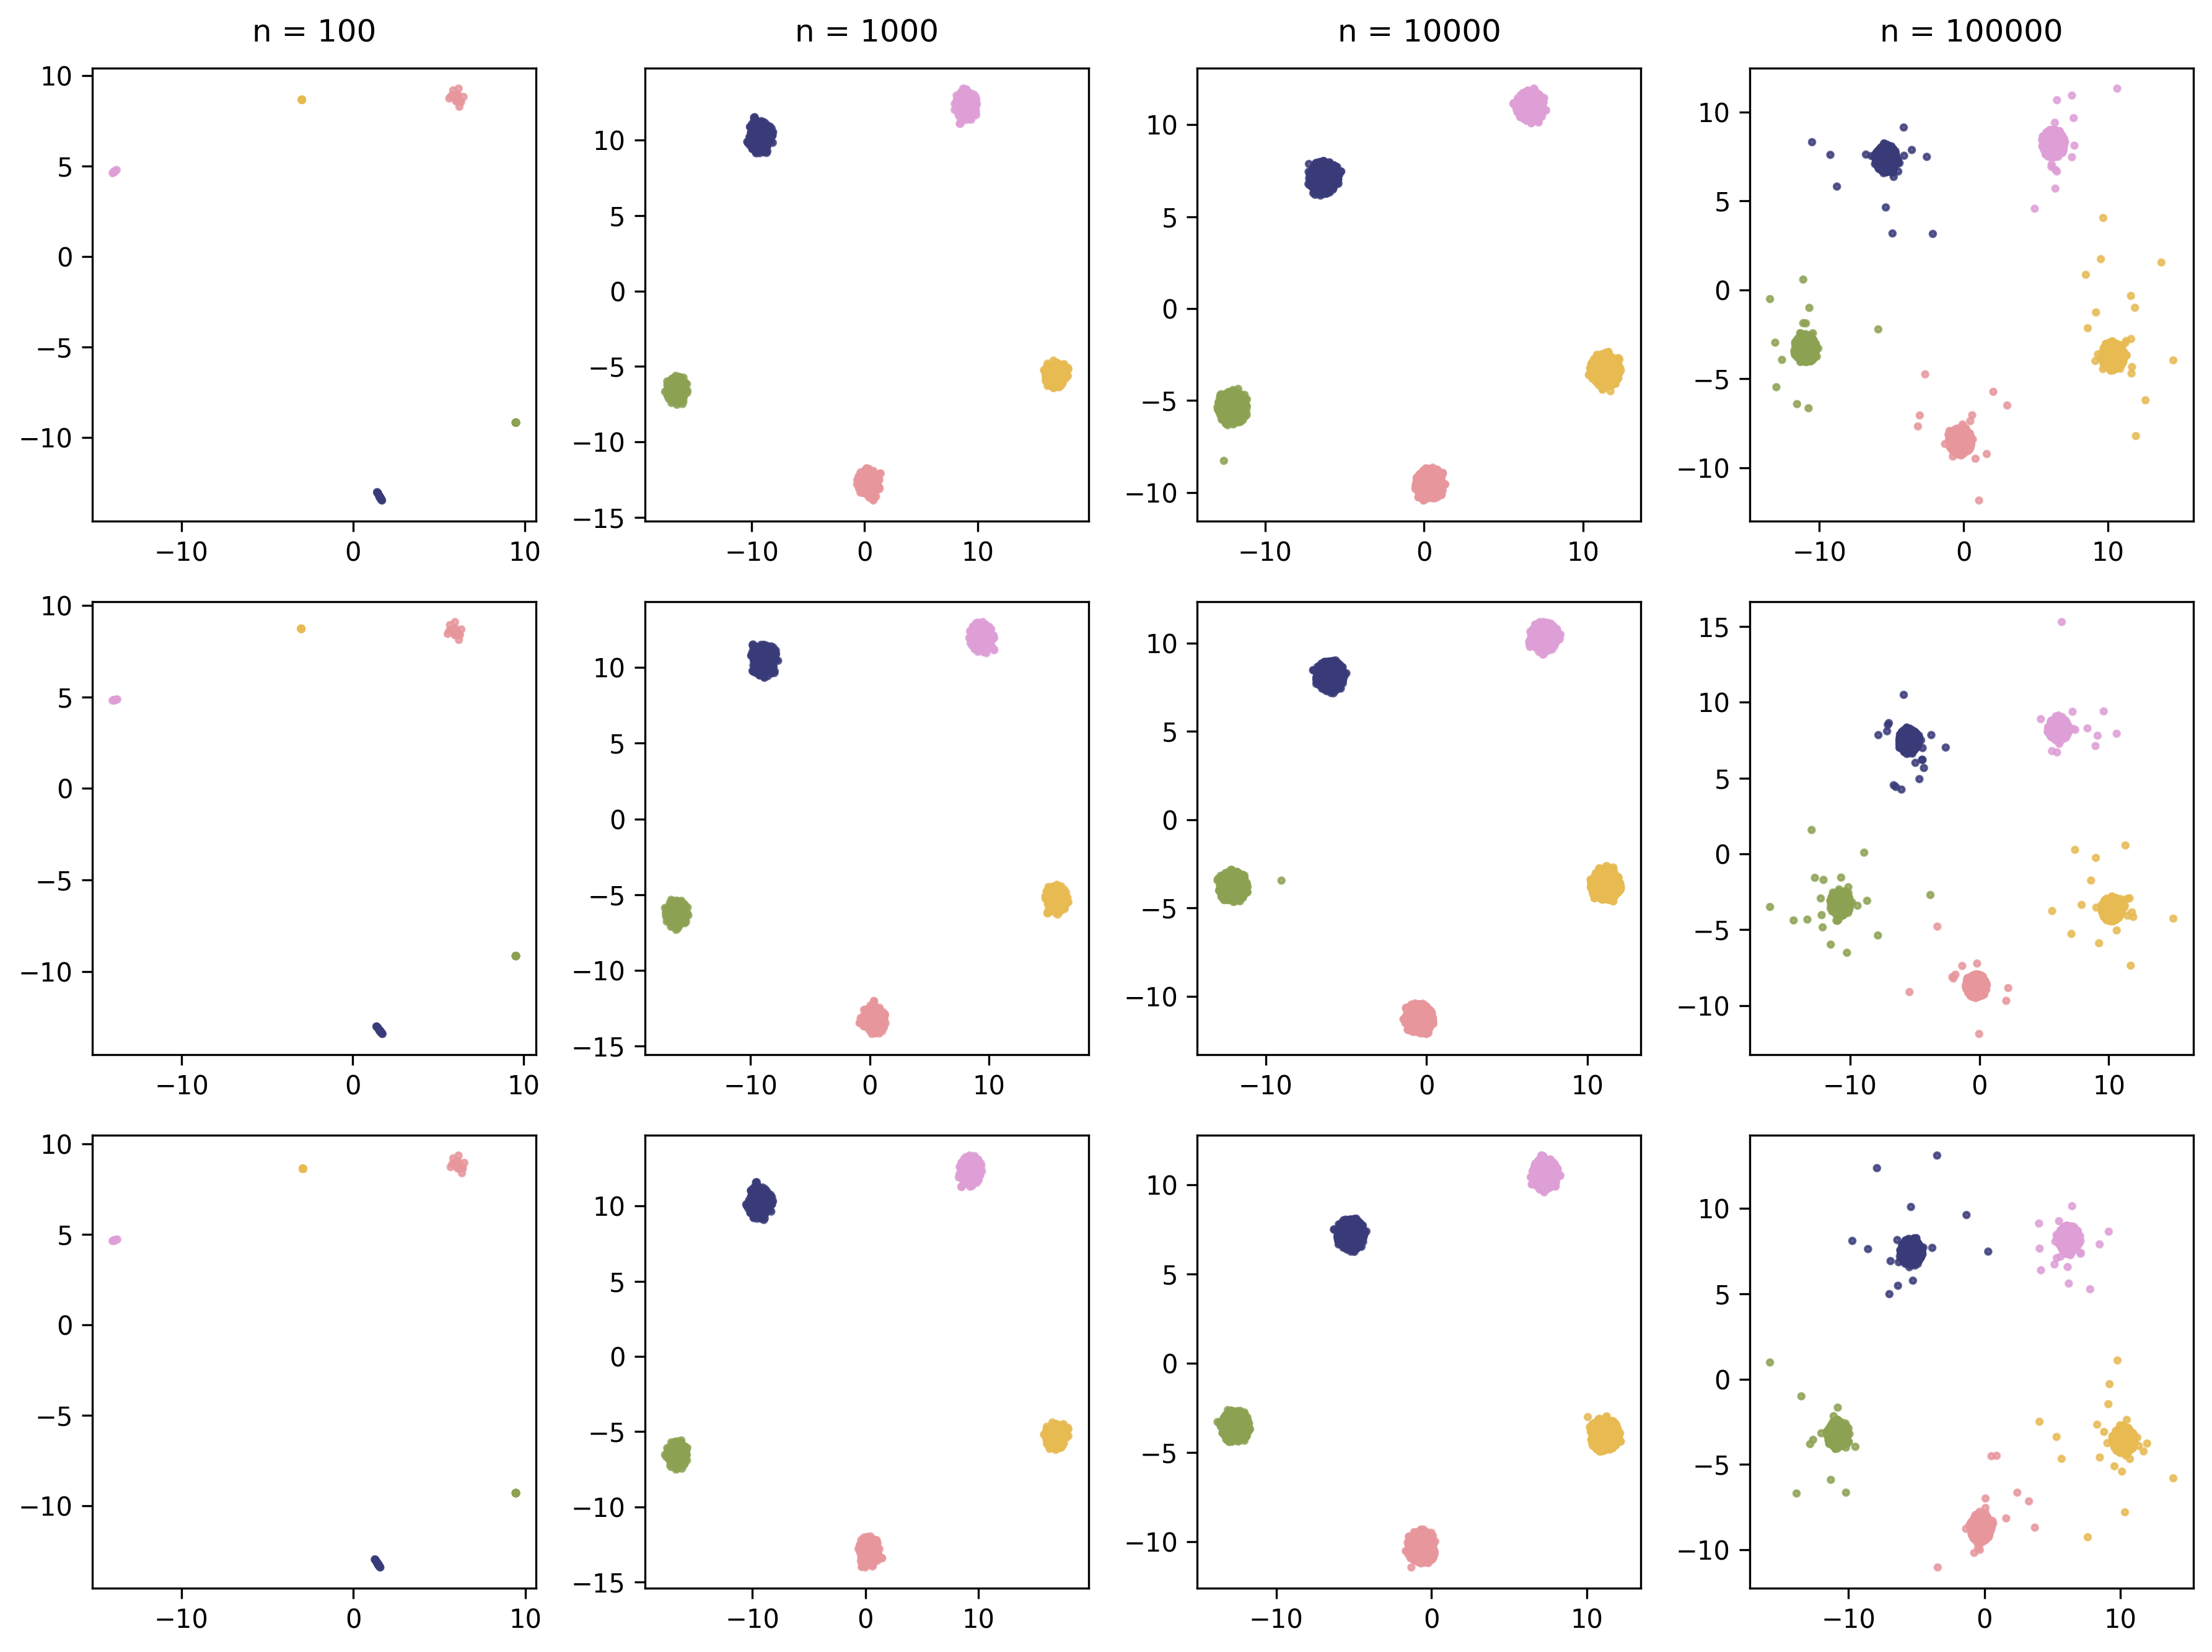
\includegraphics[width=\linewidth]{figures/rescaled/Gaussian_Mixture_rescaled_embedding_grid.png}
        \caption{Using rescaled t-SNE. Data generated from mixture of five Gaussian distributions.}
    \label{fig:Gaussian-rescaled}
\end{figure}

In the real world, things are more complicated. 

\begin{figure}[h]
    \centering 
        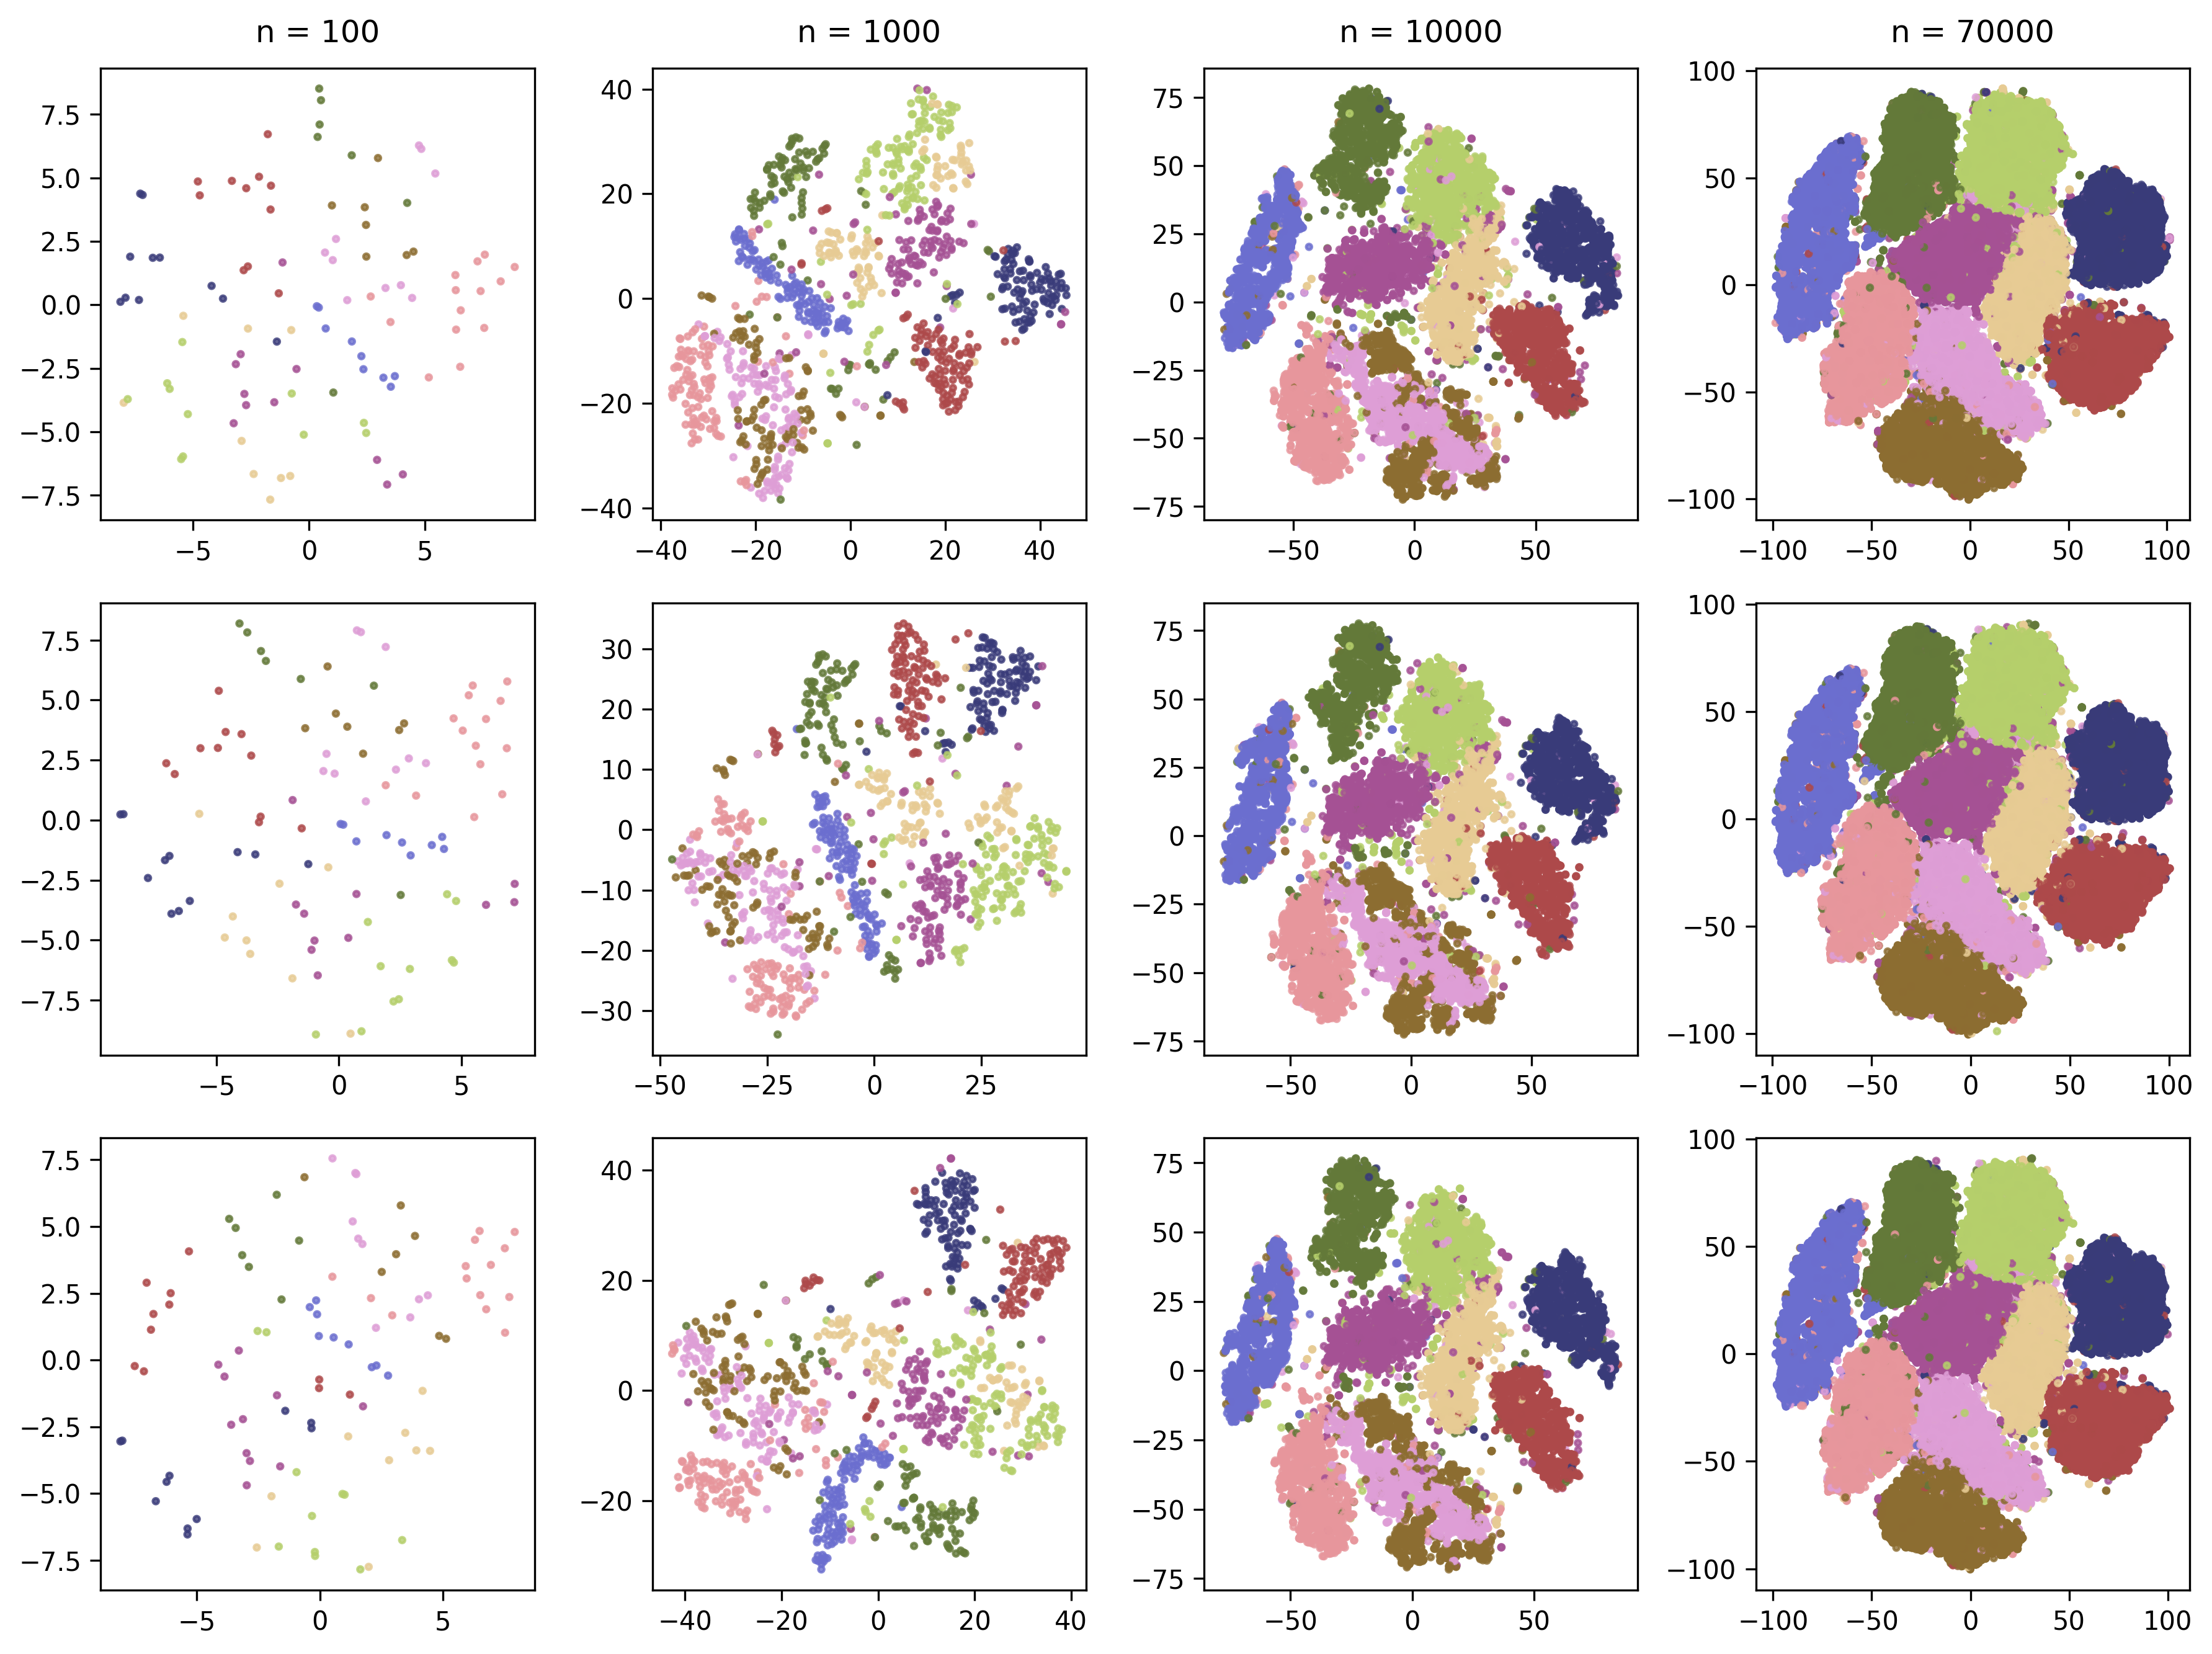
\includegraphics[width=\linewidth]{figures/rescaled/MNIST_standard_embedding_grid.png}
        \caption{Using standard t-SNE. Data sampled randomly from MNIST.}
    \label{fig:MNIST-standard}
\end{figure}

\begin{figure}[h]
    \centering 
        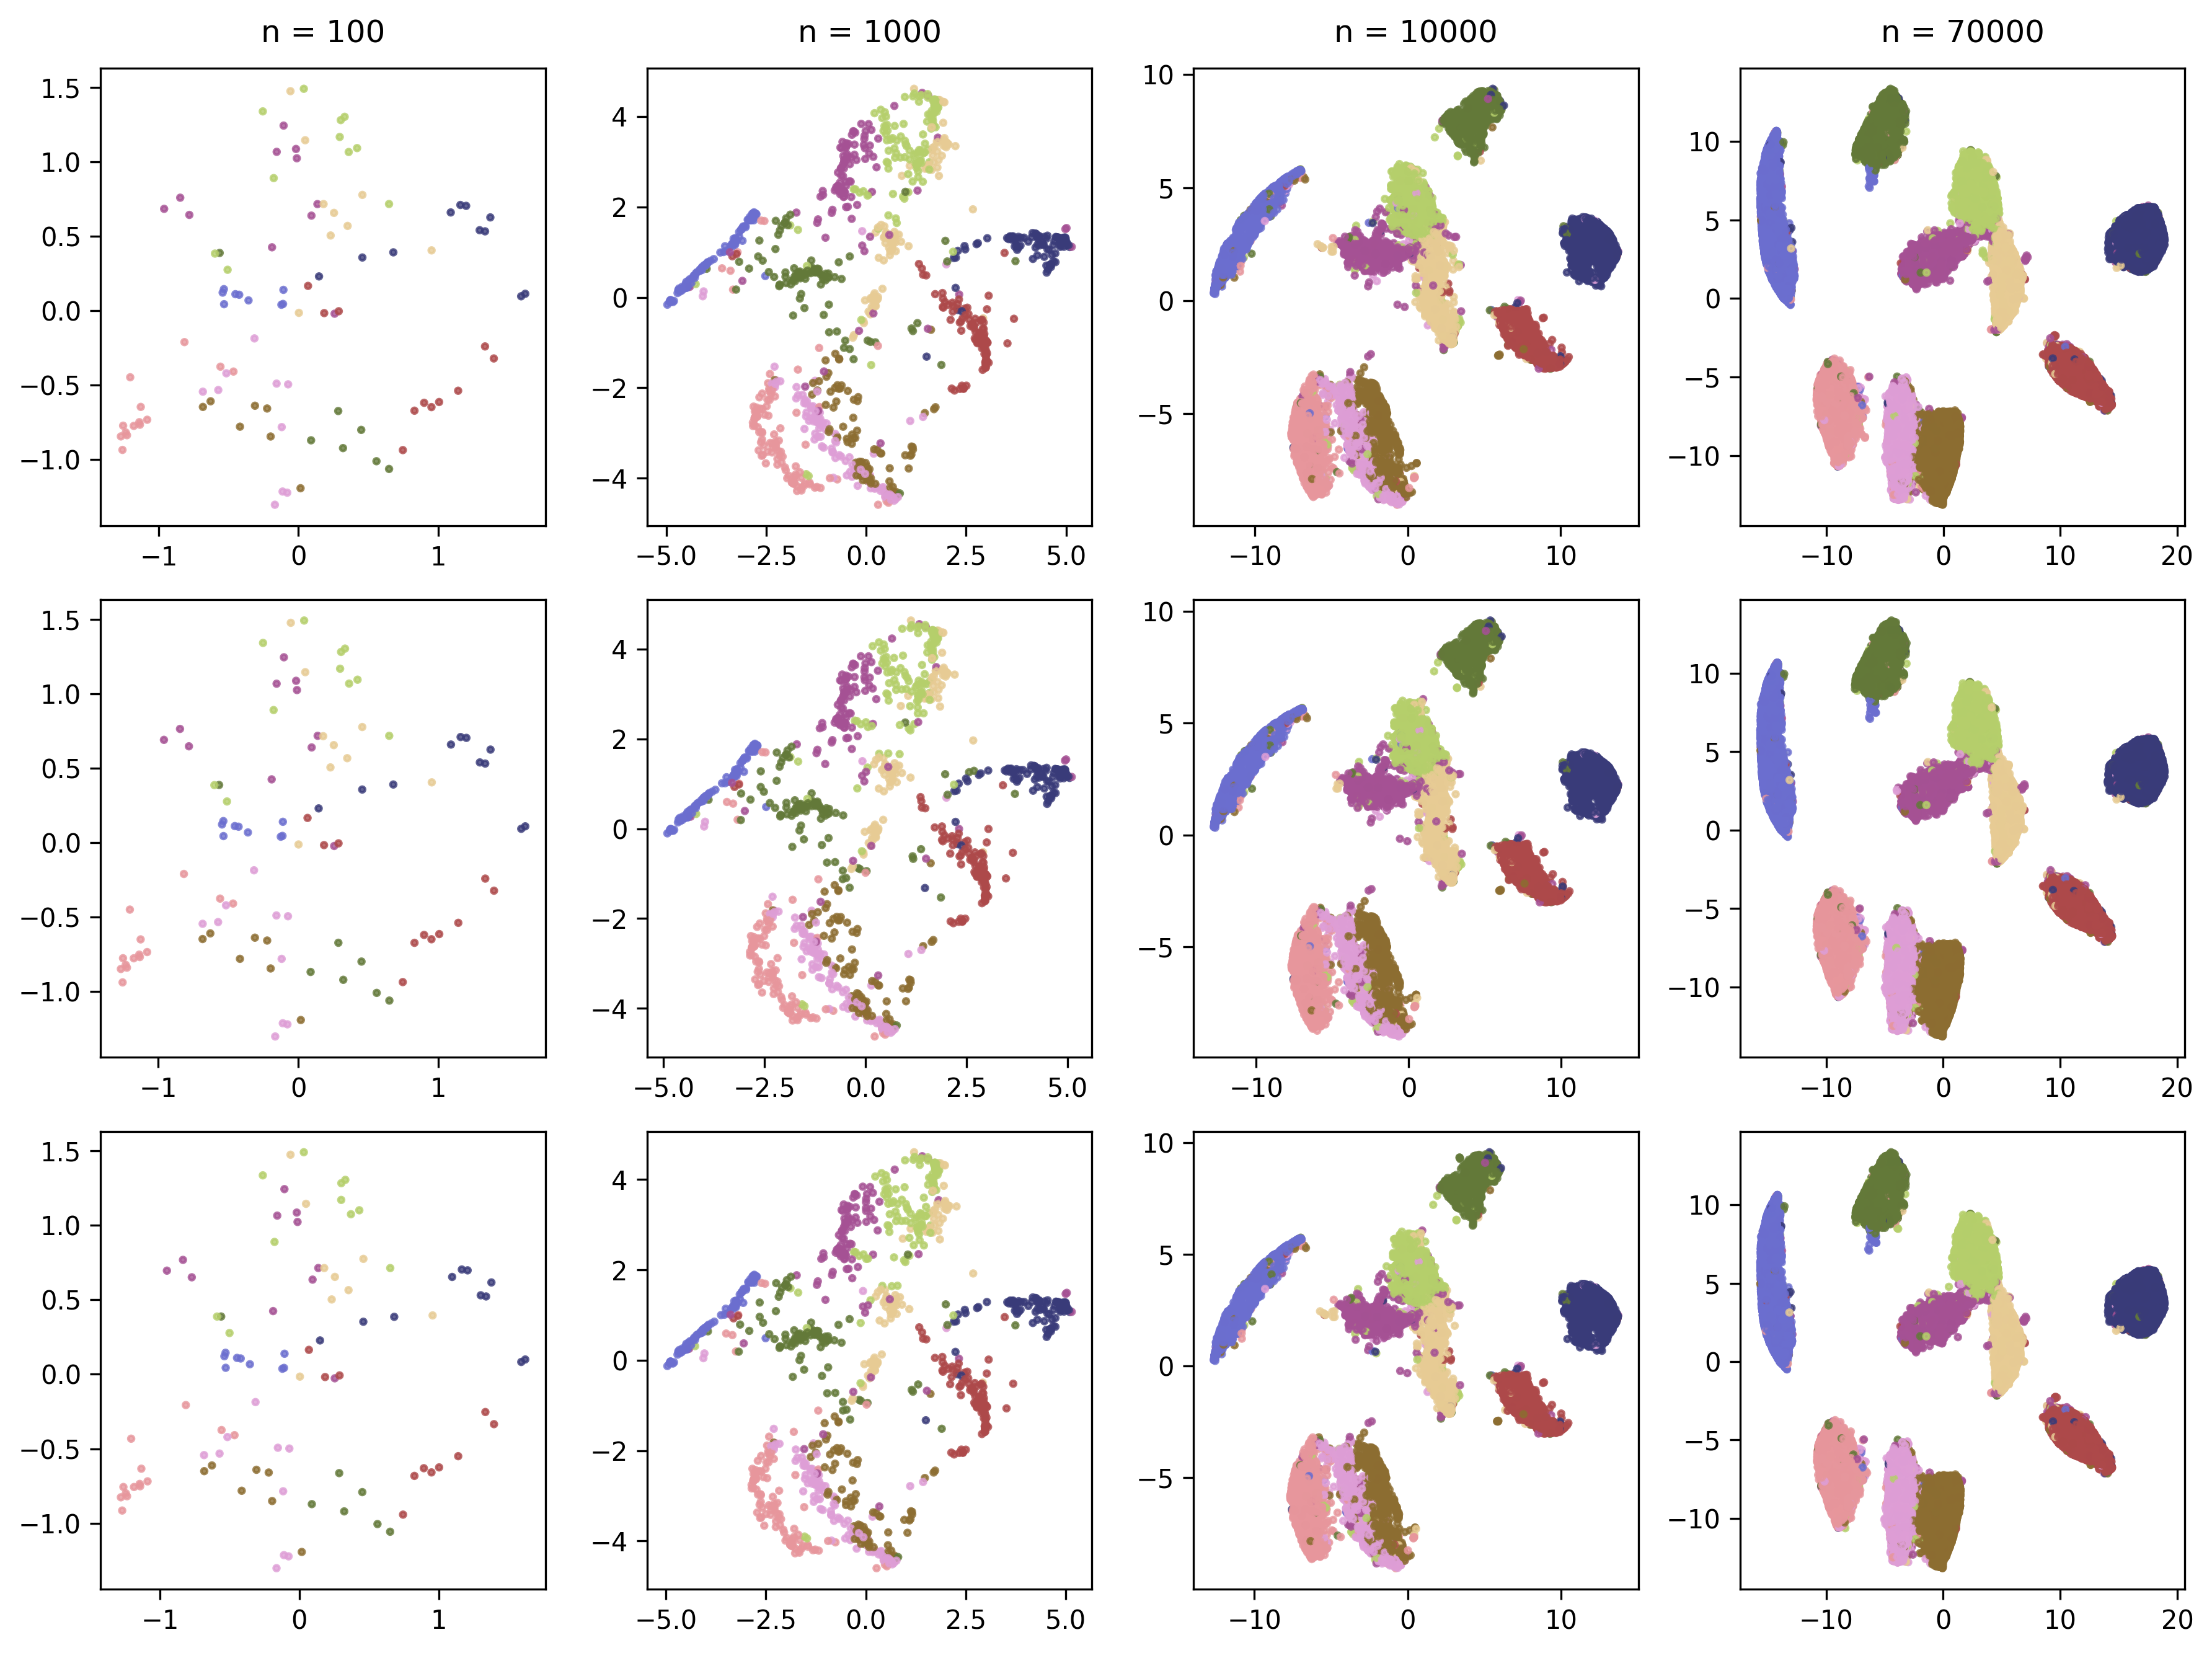
\includegraphics[width=\linewidth]{figures/rescaled/MNIST_rescaled_embedding_grid.png}
        \caption{Using rescaled t-SNE. Data sampled randomly from MNIST.}
    \label{fig:MNIST-rescaled}
\end{figure}
\newpage 
\section{Perplexity}
We look at standard perplexity values as well as adaptive ones. 
\begin{figure}[h]
    \centering 
        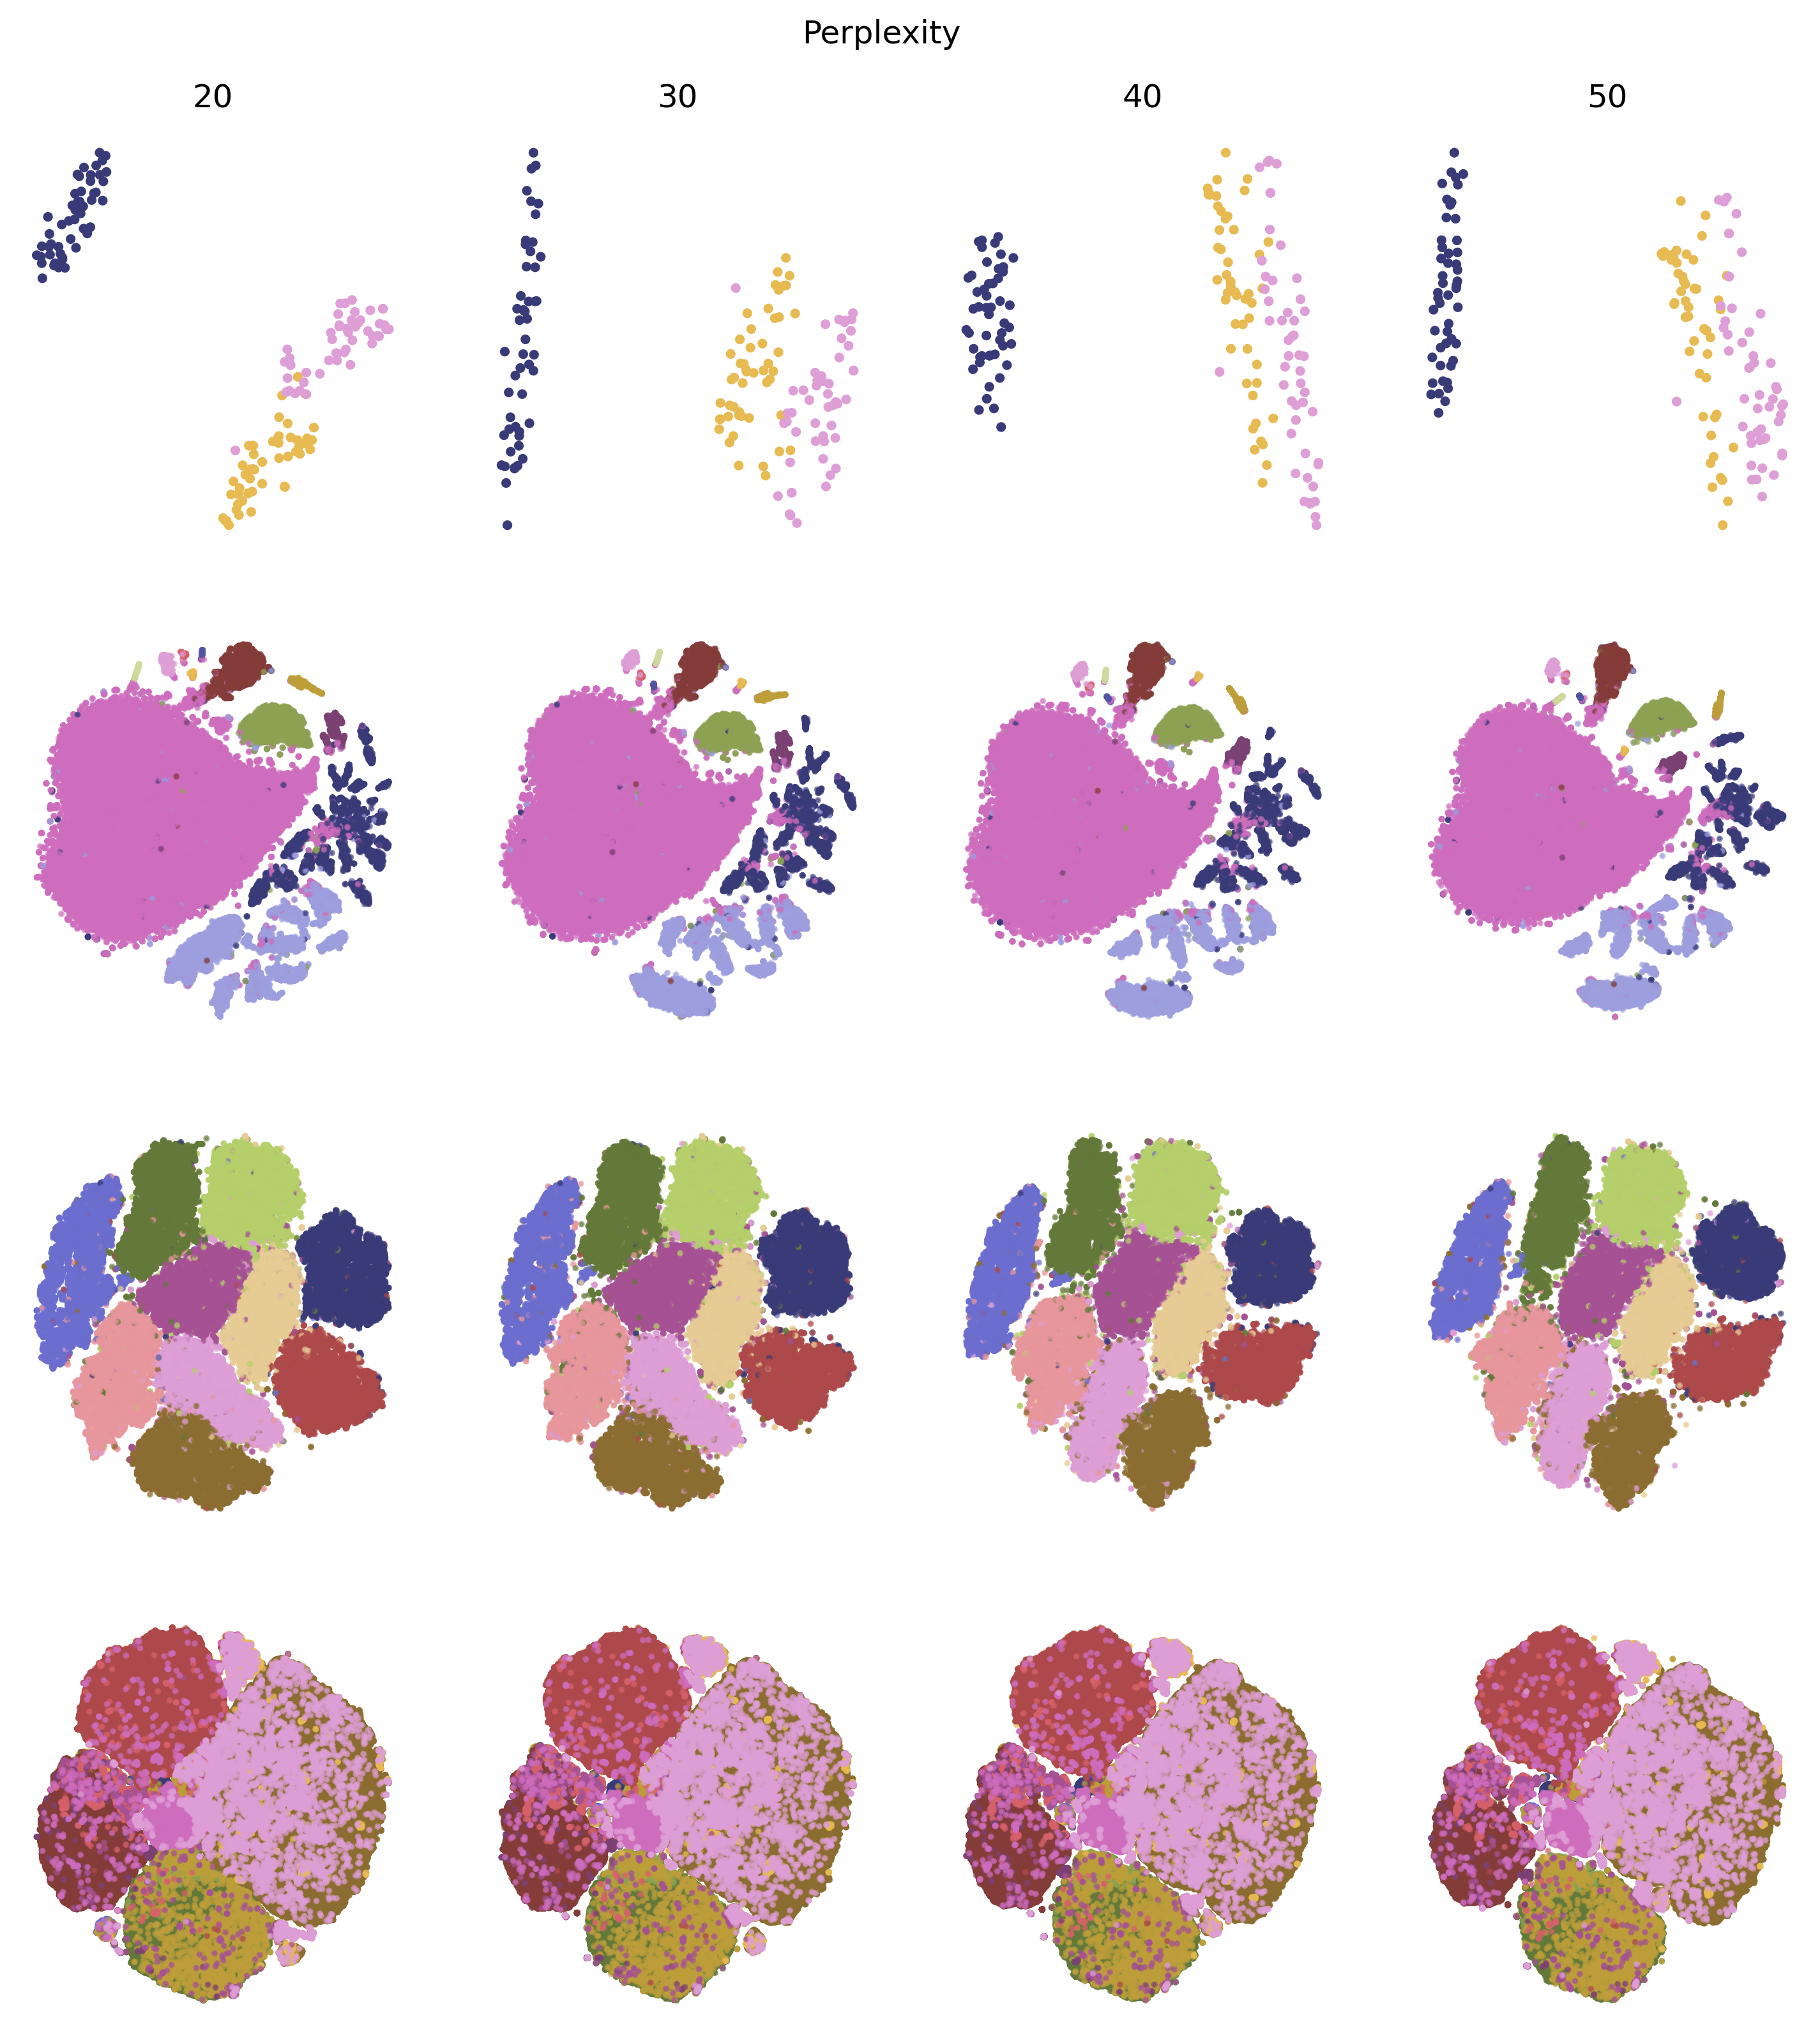
\includegraphics[width=\linewidth]{../code/figures/perp_fixed_embedding_grid_tab20b.png}
        \caption{Standard values for perplexity on different datasets. \comment{put this in the appendix}}
    \label{fig:perp_fixed_grid}
\end{figure}

\begin{figure}[h]
    \centering 
        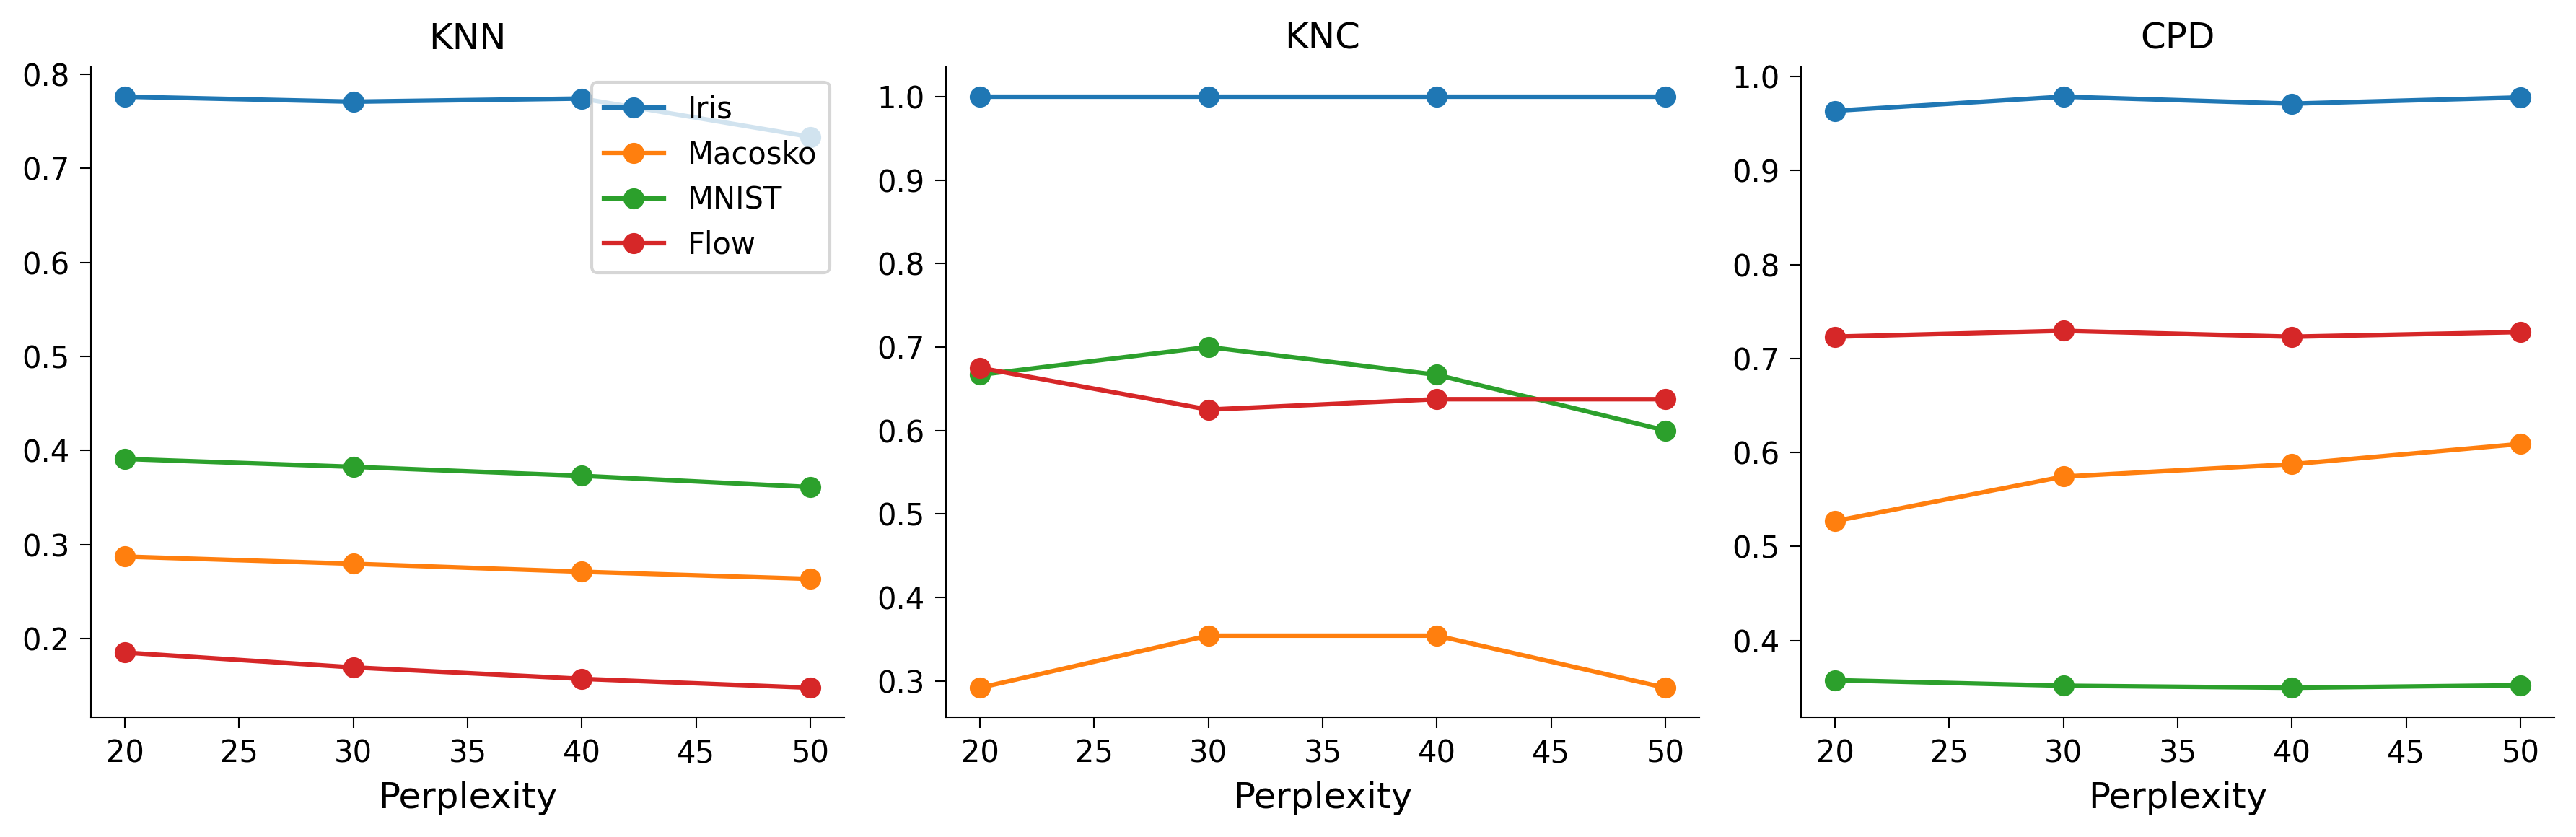
\includegraphics[width=\linewidth]{../code/figures/perp_fixed_3_quality_measures.png}
        \caption{Quality of t-SNE embeddings with different perplexities.}
    \label{fig:perp_fixed_quality}
\end{figure}
We see (\ref{fig:perp_fixed_grid}, \ref{fig:perp_fixed_quality}) that impact of perplexity on the embedding (when choosing values from the common range) is not huge. 
If anything, we see that there is a slight trade-off between global and local structure. 
The KNN values suggest that smaller perplexities lead to embeddings that preserve local structure slightly better. 
On the other hand, larger perplexity values lead to a better preservation of global structure. 
This makes sense when we think back to perplexity being a measure of the number of neighbors we consider when construction the high-dimensional affinities. 

\begin{figure}[h]
    \centering 
        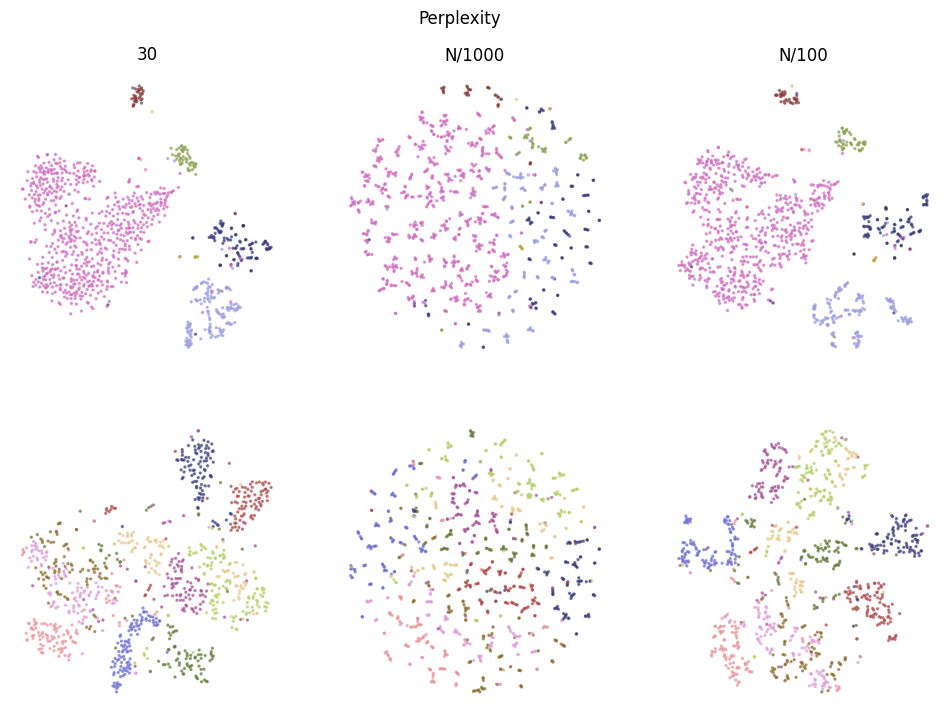
\includegraphics[width=\linewidth]{../code/figures/perp_adapt_embedding_grid_tab20b.png}
        \caption{Adaptive perplexity values on MNIST and Macosko datasets.}
    \label{fig:perp_adapt_grid}
\end{figure}

\begin{figure}[h]
    \centering 
        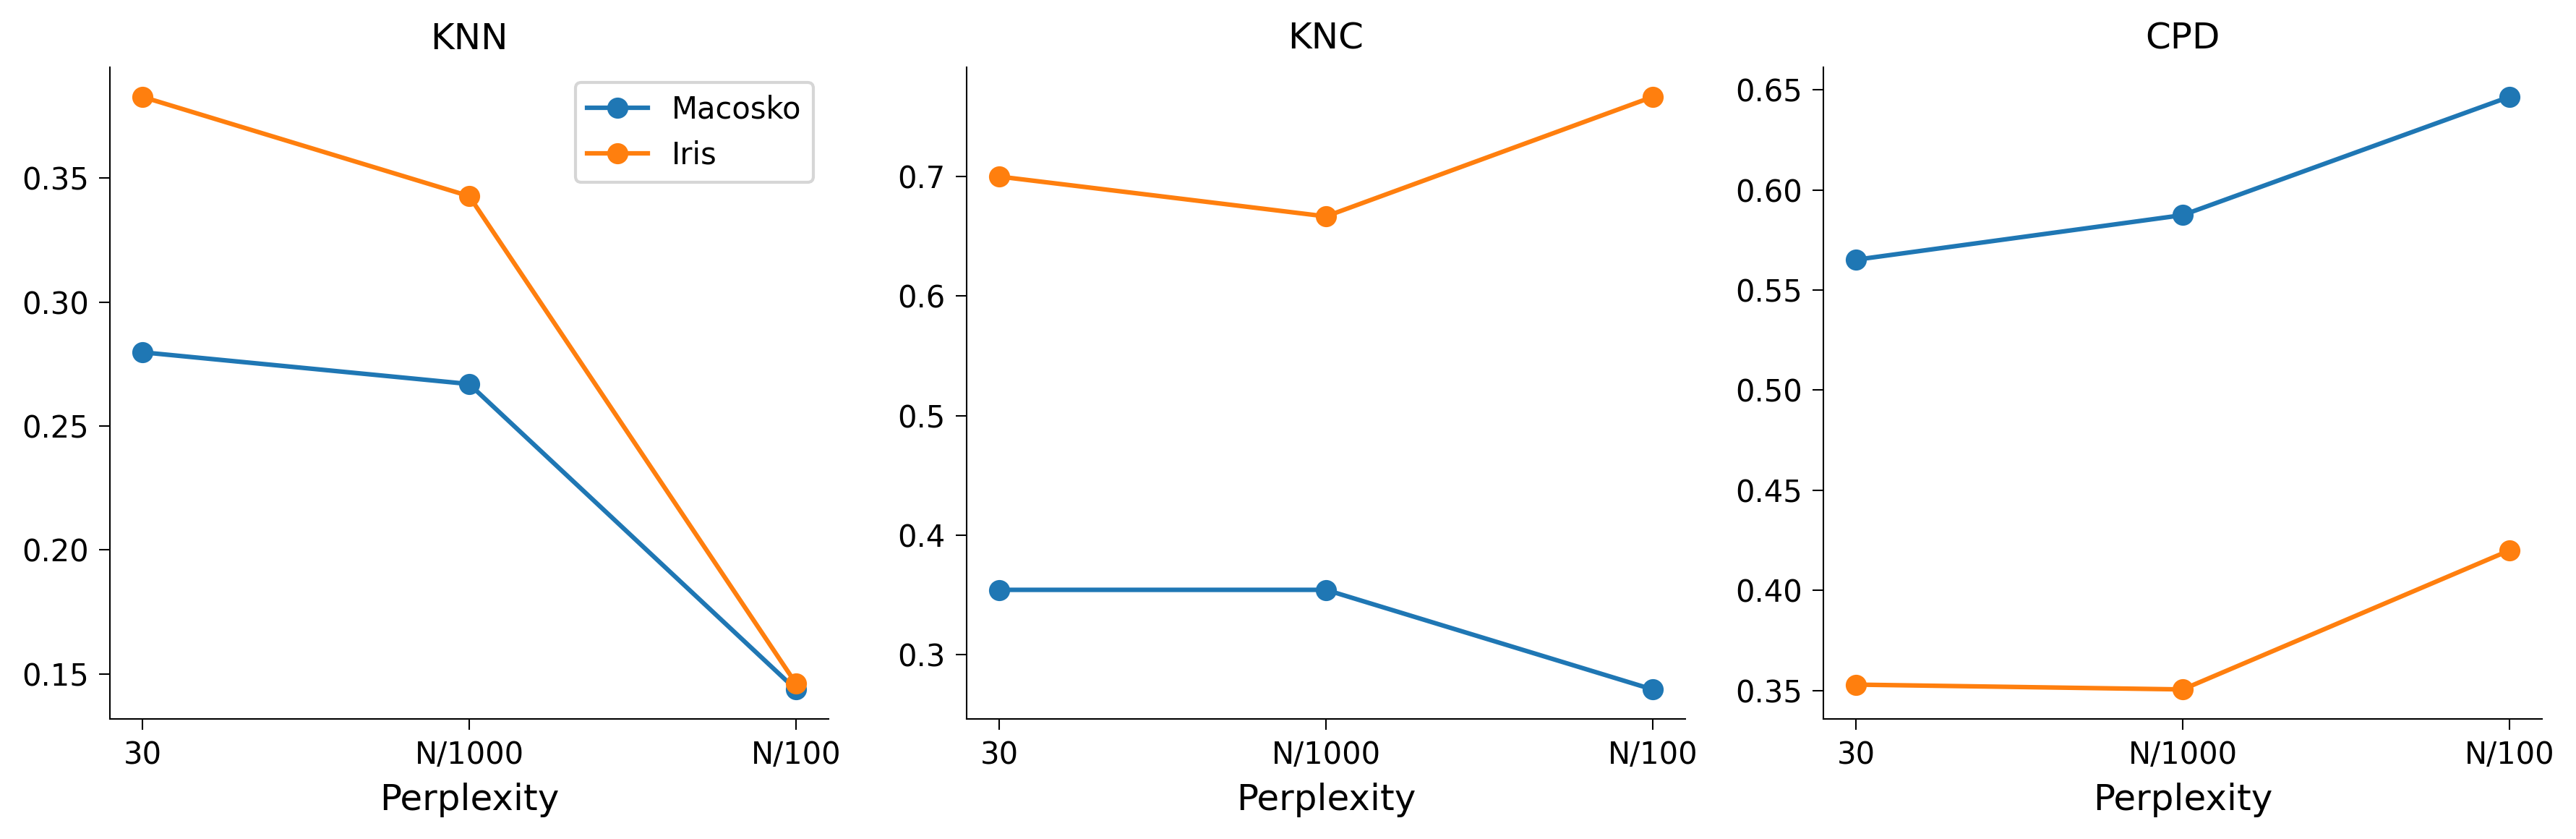
\includegraphics[width=\linewidth]{../code/figures/perp_adapt_3_quality_measures.png}
        \caption{Quality of t-SNE embeddings with different (adaptive) perplexities.}
    \label{fig:perp_adapt_quality}
\end{figure}

We basically observe the same thing with adaptive perplexity values. 
The adaptive perplexity $N/100$ suggested by \cite{KoBe19SingleCell} visually leads to embeddings that do not lead to as good of a clustering (\ref{fig:perp_adapt_grid}). 
They do however preserve local structure better (\ref{fig:perp_adapt_quality}). 
\newpage 
\section{Learning Rate}
We consider the effect of different learning rates on the embedding. We can see that for $\eta=1$, this doesn't lead to good results (apart from the global structure). The best results are achieved with the \enquote{auto} setting across datasets. 
\begin{figure}[h]
    \centering 
        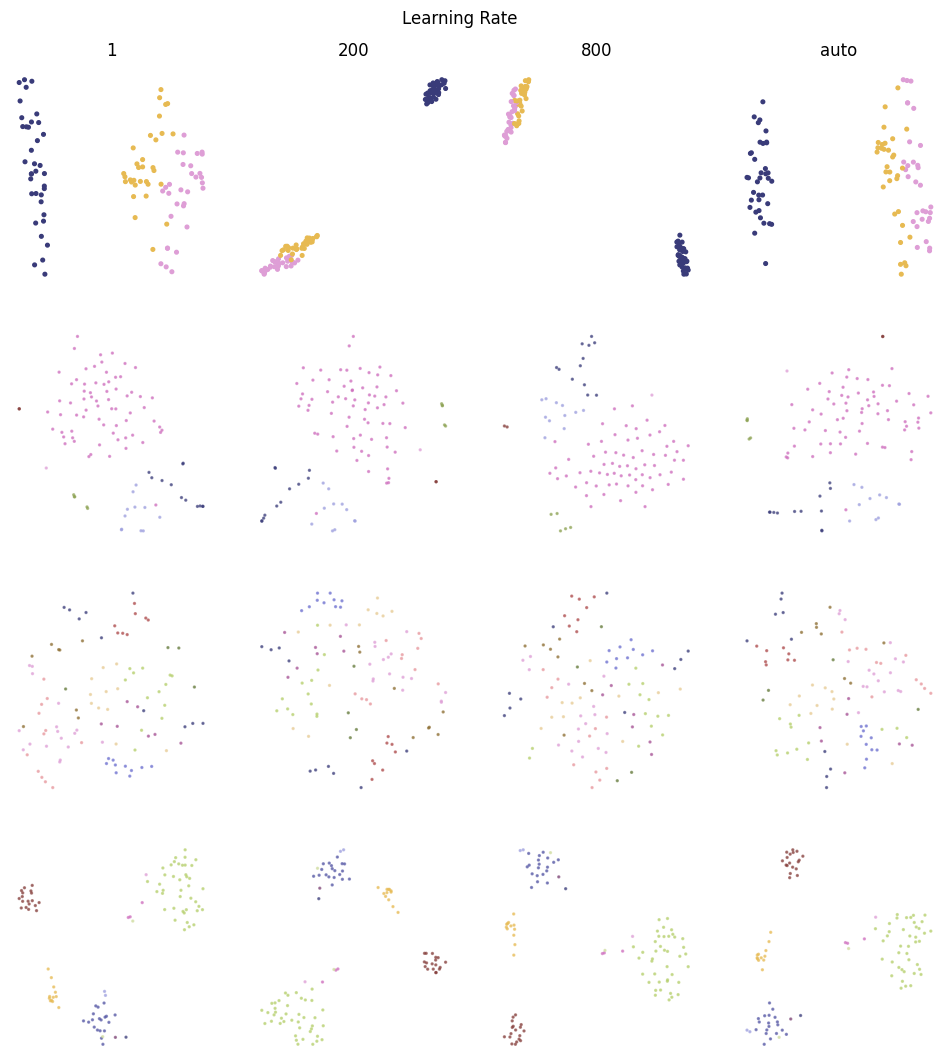
\includegraphics[width=\linewidth]{../code/figures/eta_embedding_grid_tab20b.png}
        \caption{Effect of different learning rates on the embedding.}
    \label{fig:eta_grid}
\end{figure} 

\begin{figure}[h]
    \centering 
        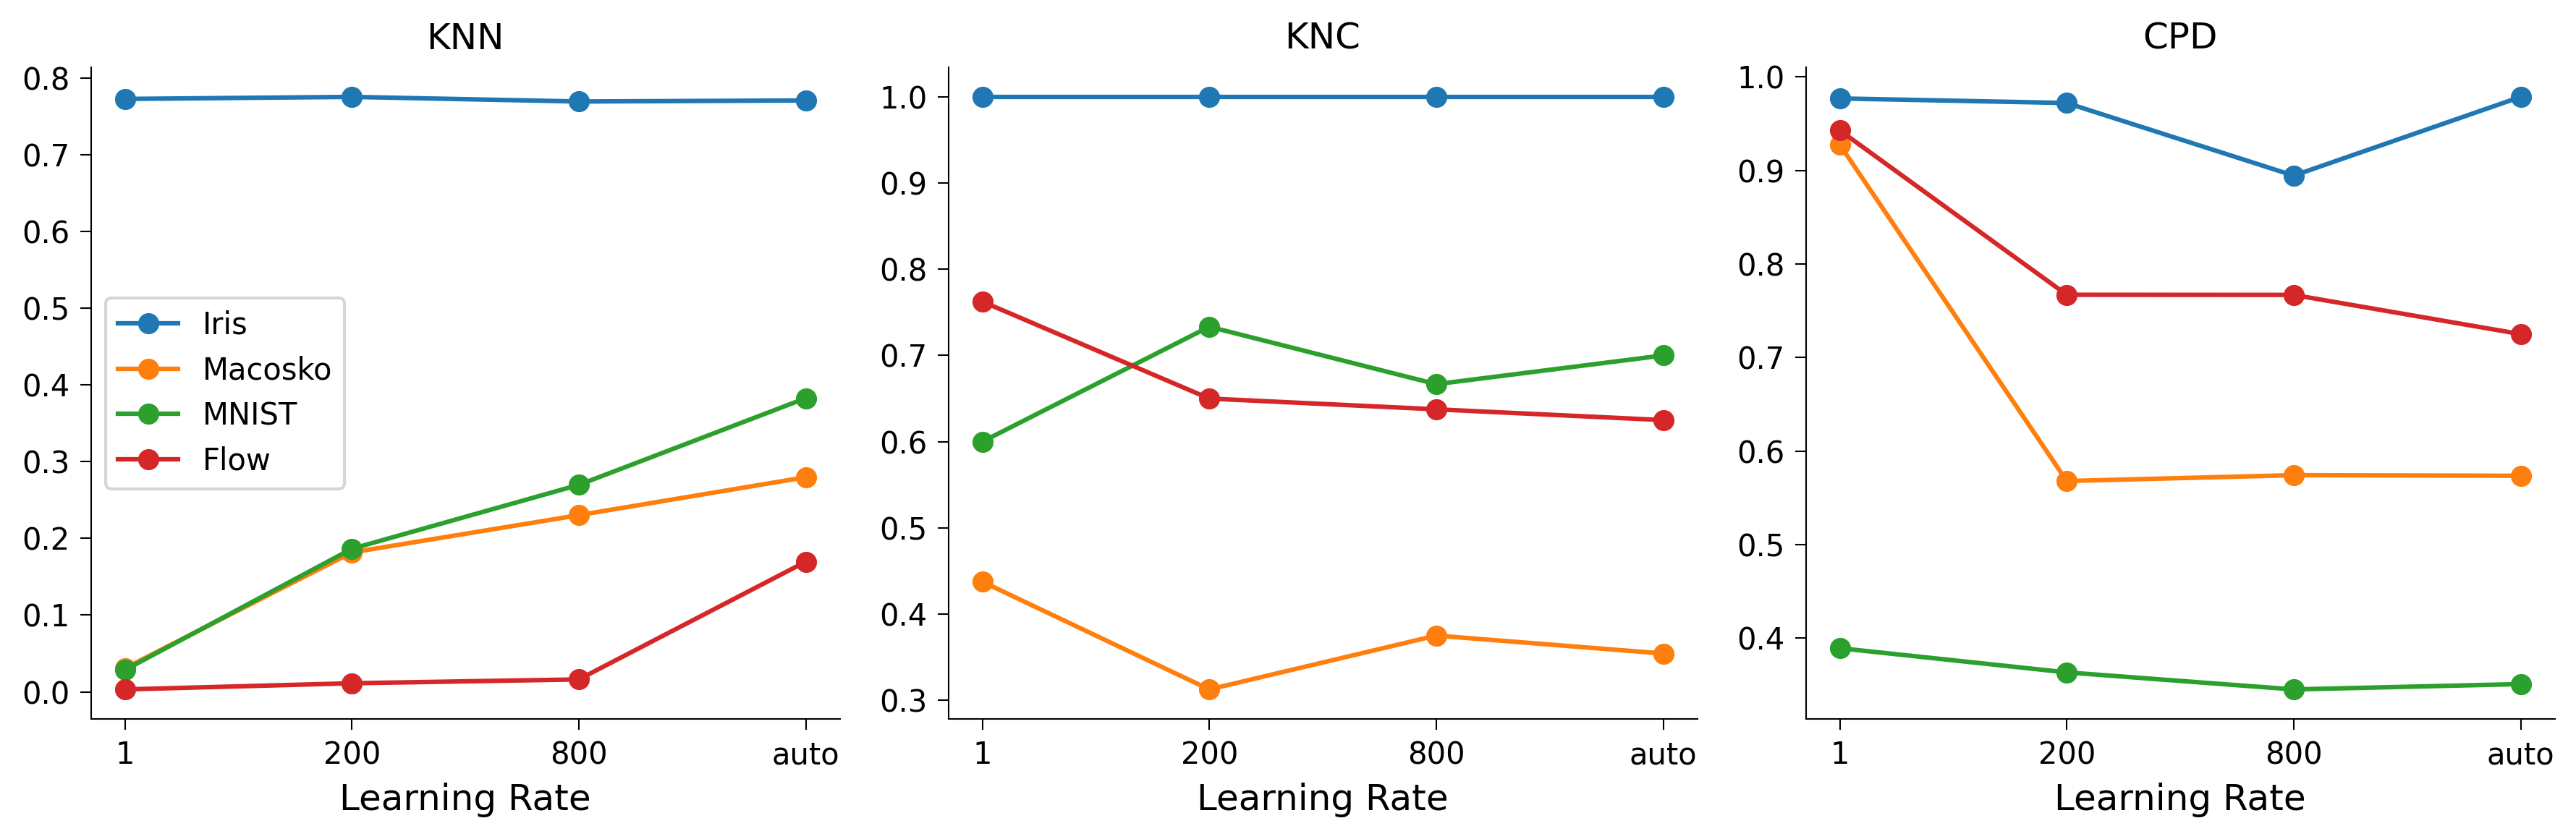
\includegraphics[width=\linewidth]{../code/figures/eta_3_quality_measures.png}
        \caption{Quality of t-SNE embeddings with different learning rates.}
    \label{fig:eta_quality}
\end{figure}
As for the KL divergence plots, we see that squiggly lines occur when using too large learning rates on the small Iris datset (\ref{fig:eta_kld}). This phenomenon is commonly seen in machine learning - oscillation because the high learning rate makes us overshoot. 
\begin{figure}[h]
    \centering 
        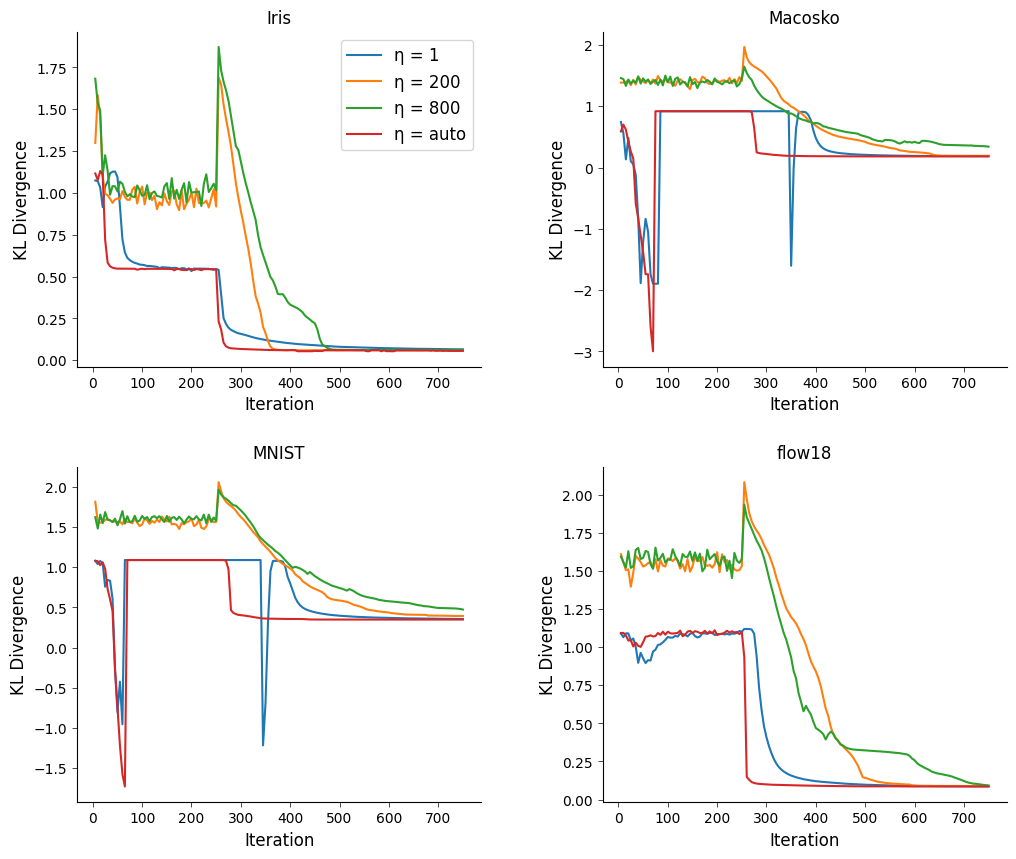
\includegraphics[width=\linewidth]{../code/figures/eta_kl_divergences_grid.png}
        \caption{KLD of t-SNE embeddings with different learning rates.}
    \label{fig:eta_kld}
\end{figure}
\newpage 
\section{Early Exaggeration}
We begin by examining the early exaggeration factor. 

\begin{figure}[h]
    \centering 
        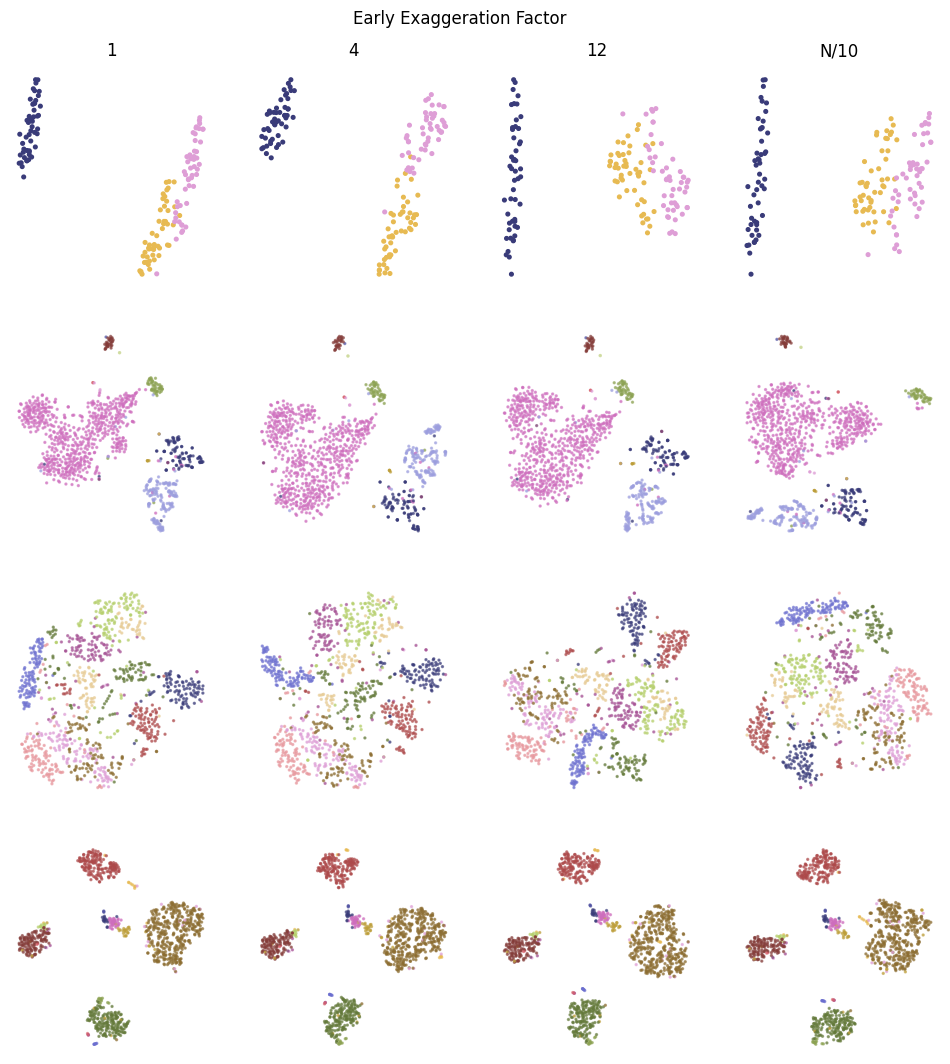
\includegraphics[width=\linewidth]{../code/figures/alpha_embedding_grid_tab20b.png}
        \caption{t-SNE embeddings with different EE factors.}
    \label{fig:alpha_grid}
\end{figure}

We can see in \ref{fig:alpha_grid} that EE factors 4 and 12 work best. For $\alpha=1$, some of the clusters aren't together in the Macosko dataset, for example the light green one. This is also the case for the MNIST dataset - the blue and brown clusters are separated in the $\alpha = N/10$ case. We conclude that values $\alpha=4$ to $\alpha=12$ work best. 

\begin{figure}[h]
    \centering 
        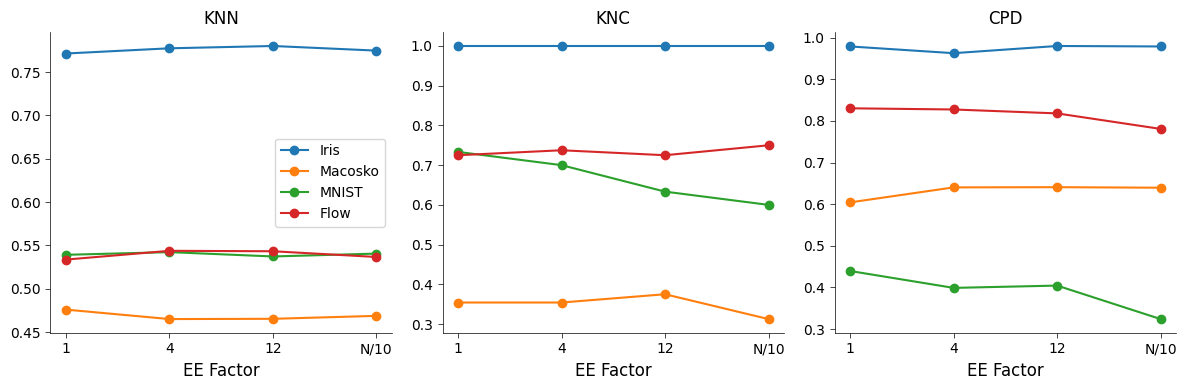
\includegraphics[width=\linewidth]{../code/figures/alpha_3_quality_measures.png}
        \caption{Quality of t-SNE embeddings with different EE factors.}
    \label{fig:alpha_quality}
\end{figure}

\begin{figure}[h]
    \centering 
        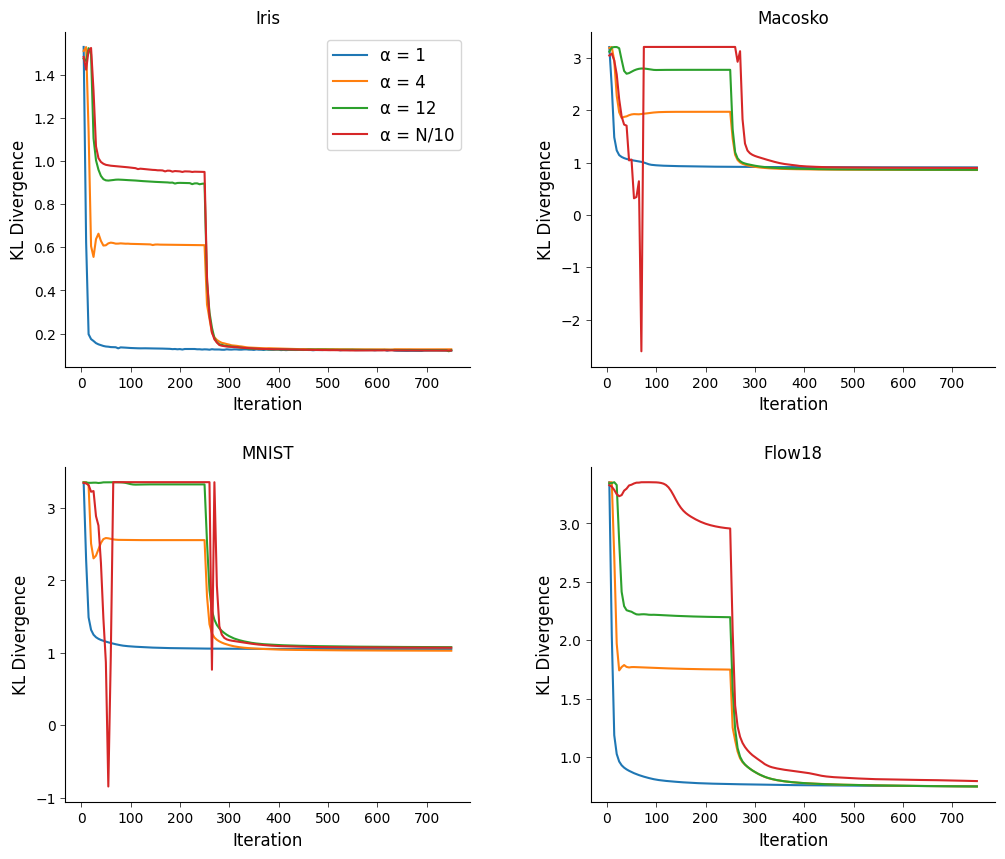
\includegraphics[width=\linewidth]{../code/figures/alpha_kl_divergences_grid.png}
        \caption{KLD of t-SNE embeddings with different EE factors. \comment{do I actually want to include this? does it even make sense?}}
    \label{fig:alpha_kld}
\end{figure}


It is also interesting to look at the length of EE. We also try out different values for this. 
\begin{figure}[h]
    \centering 
        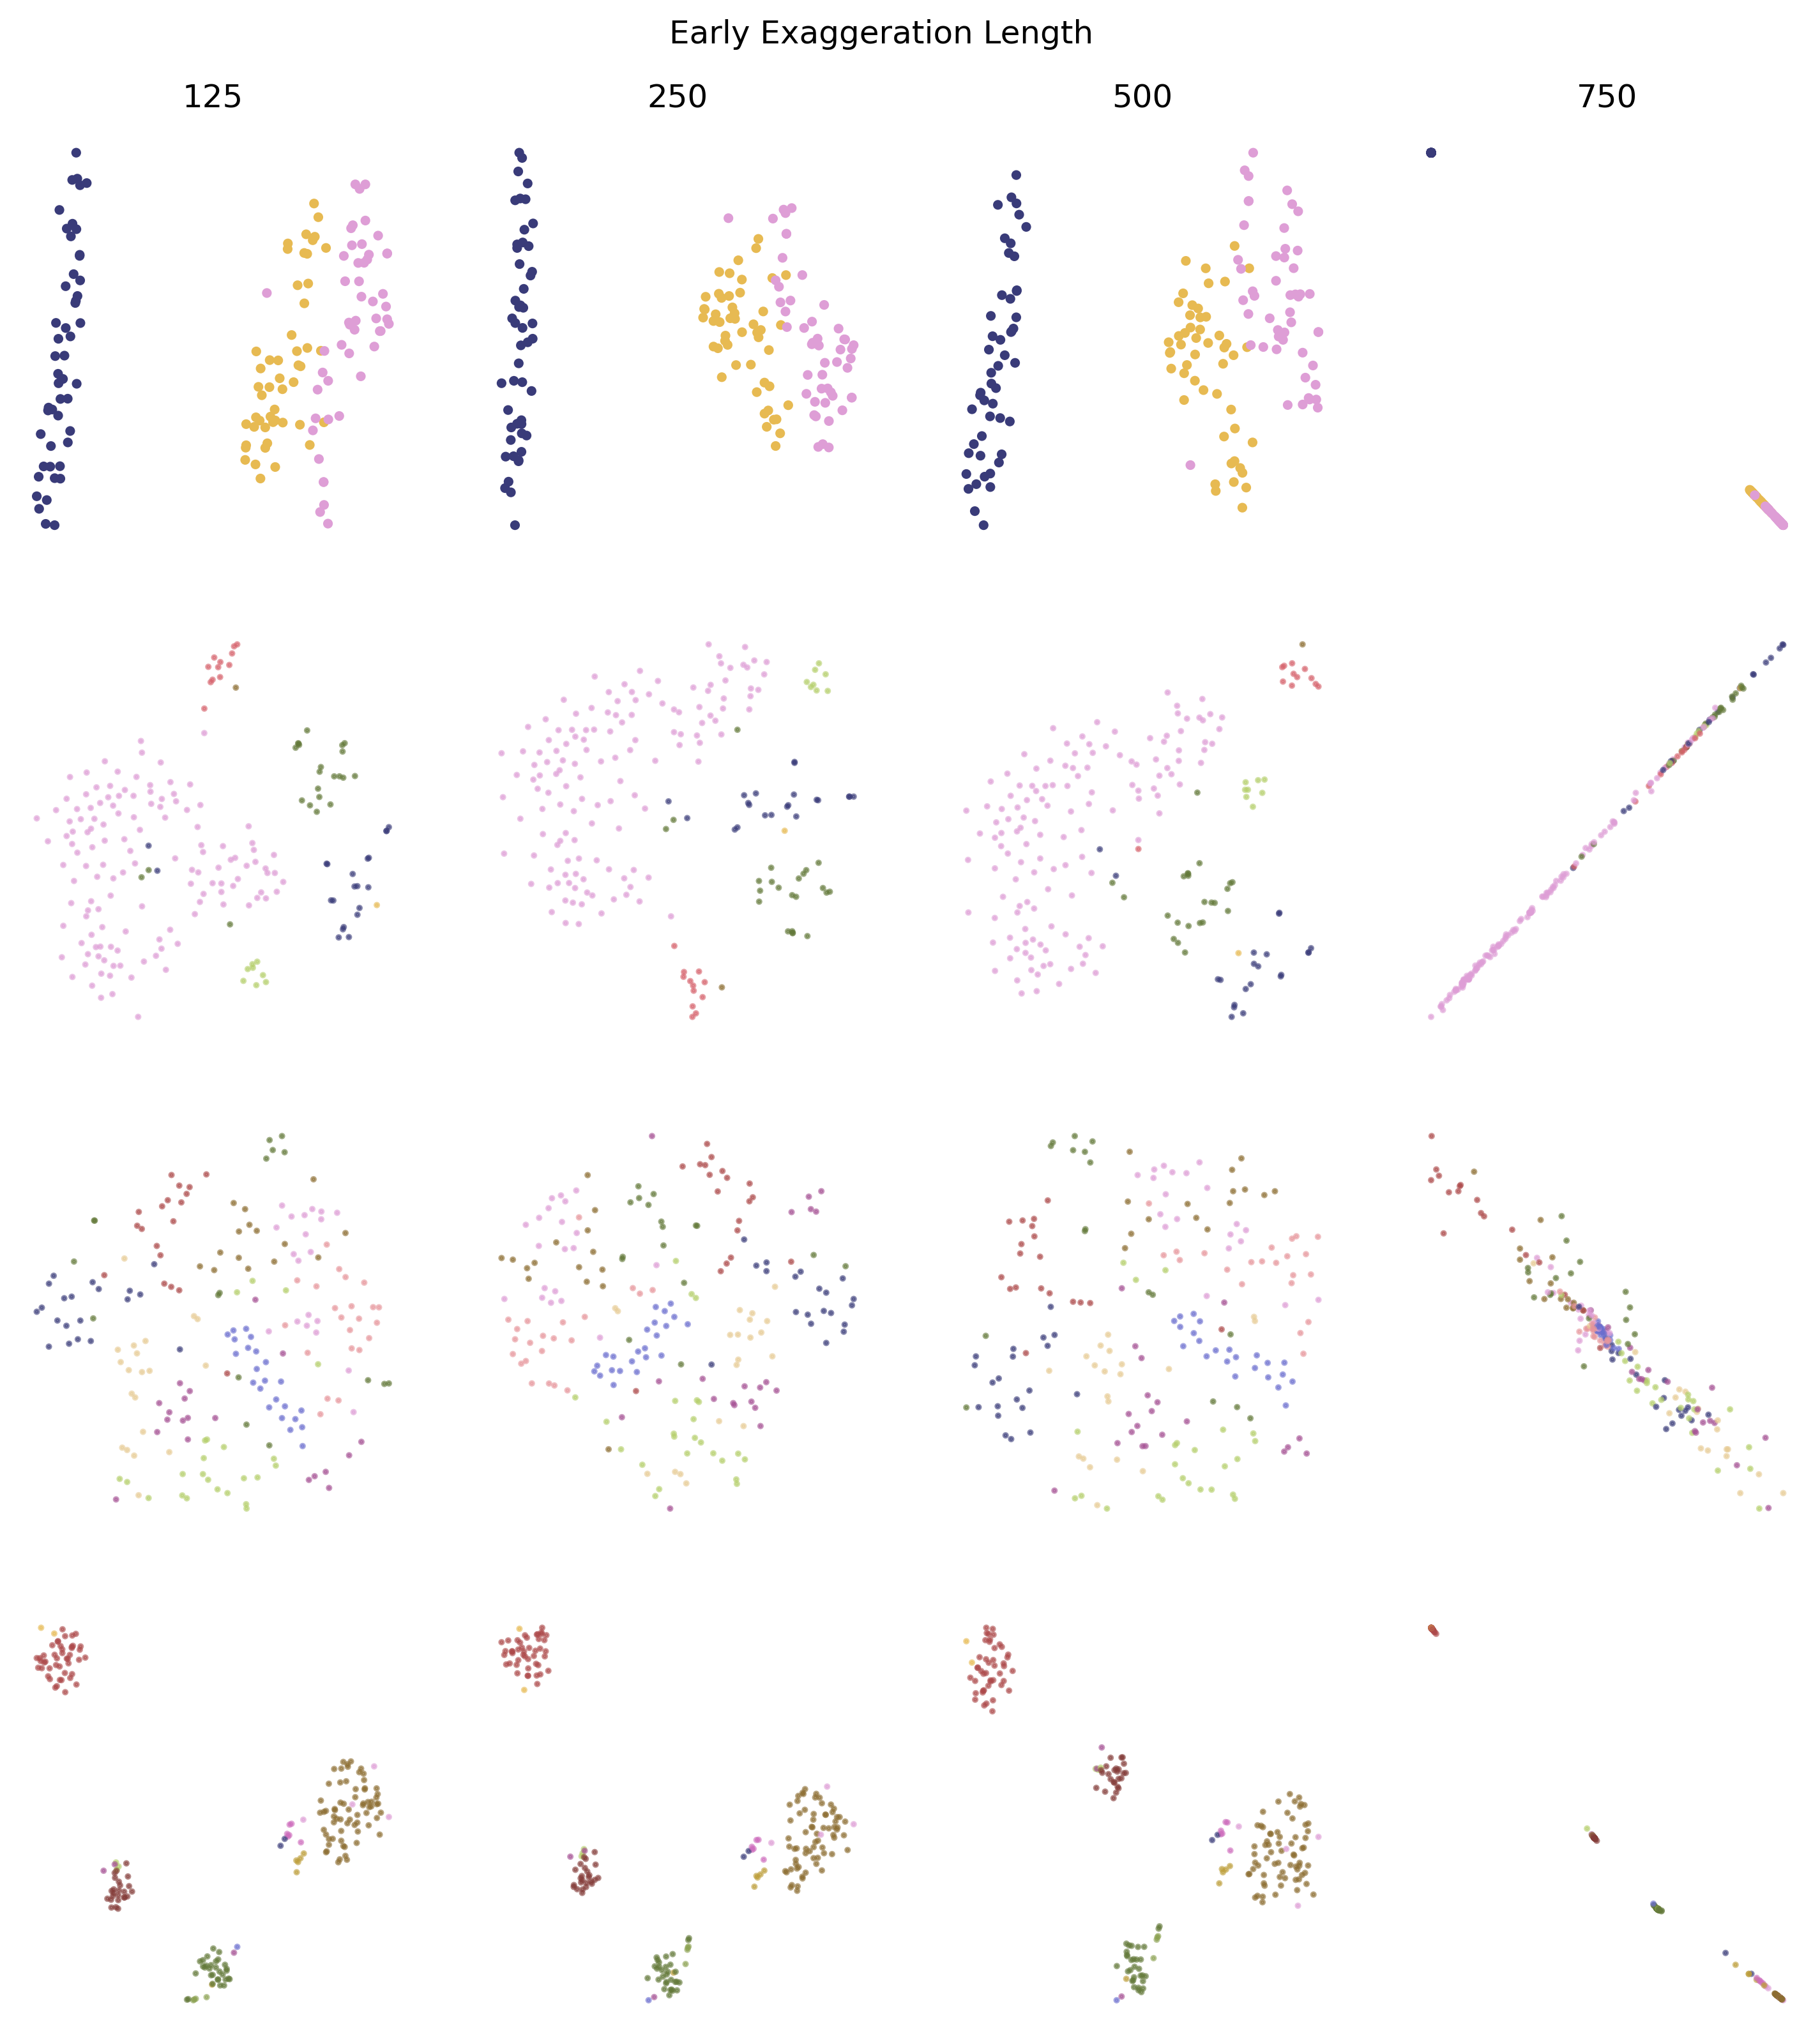
\includegraphics[width=\linewidth]{../code/figures/ee_length_embedding_grid_tab20b.png}
        \caption{t-SNE embeddings with different EE lengths.}
    \label{fig:EE_length_grid}
\end{figure}

\begin{figure}[h]
    \centering 
        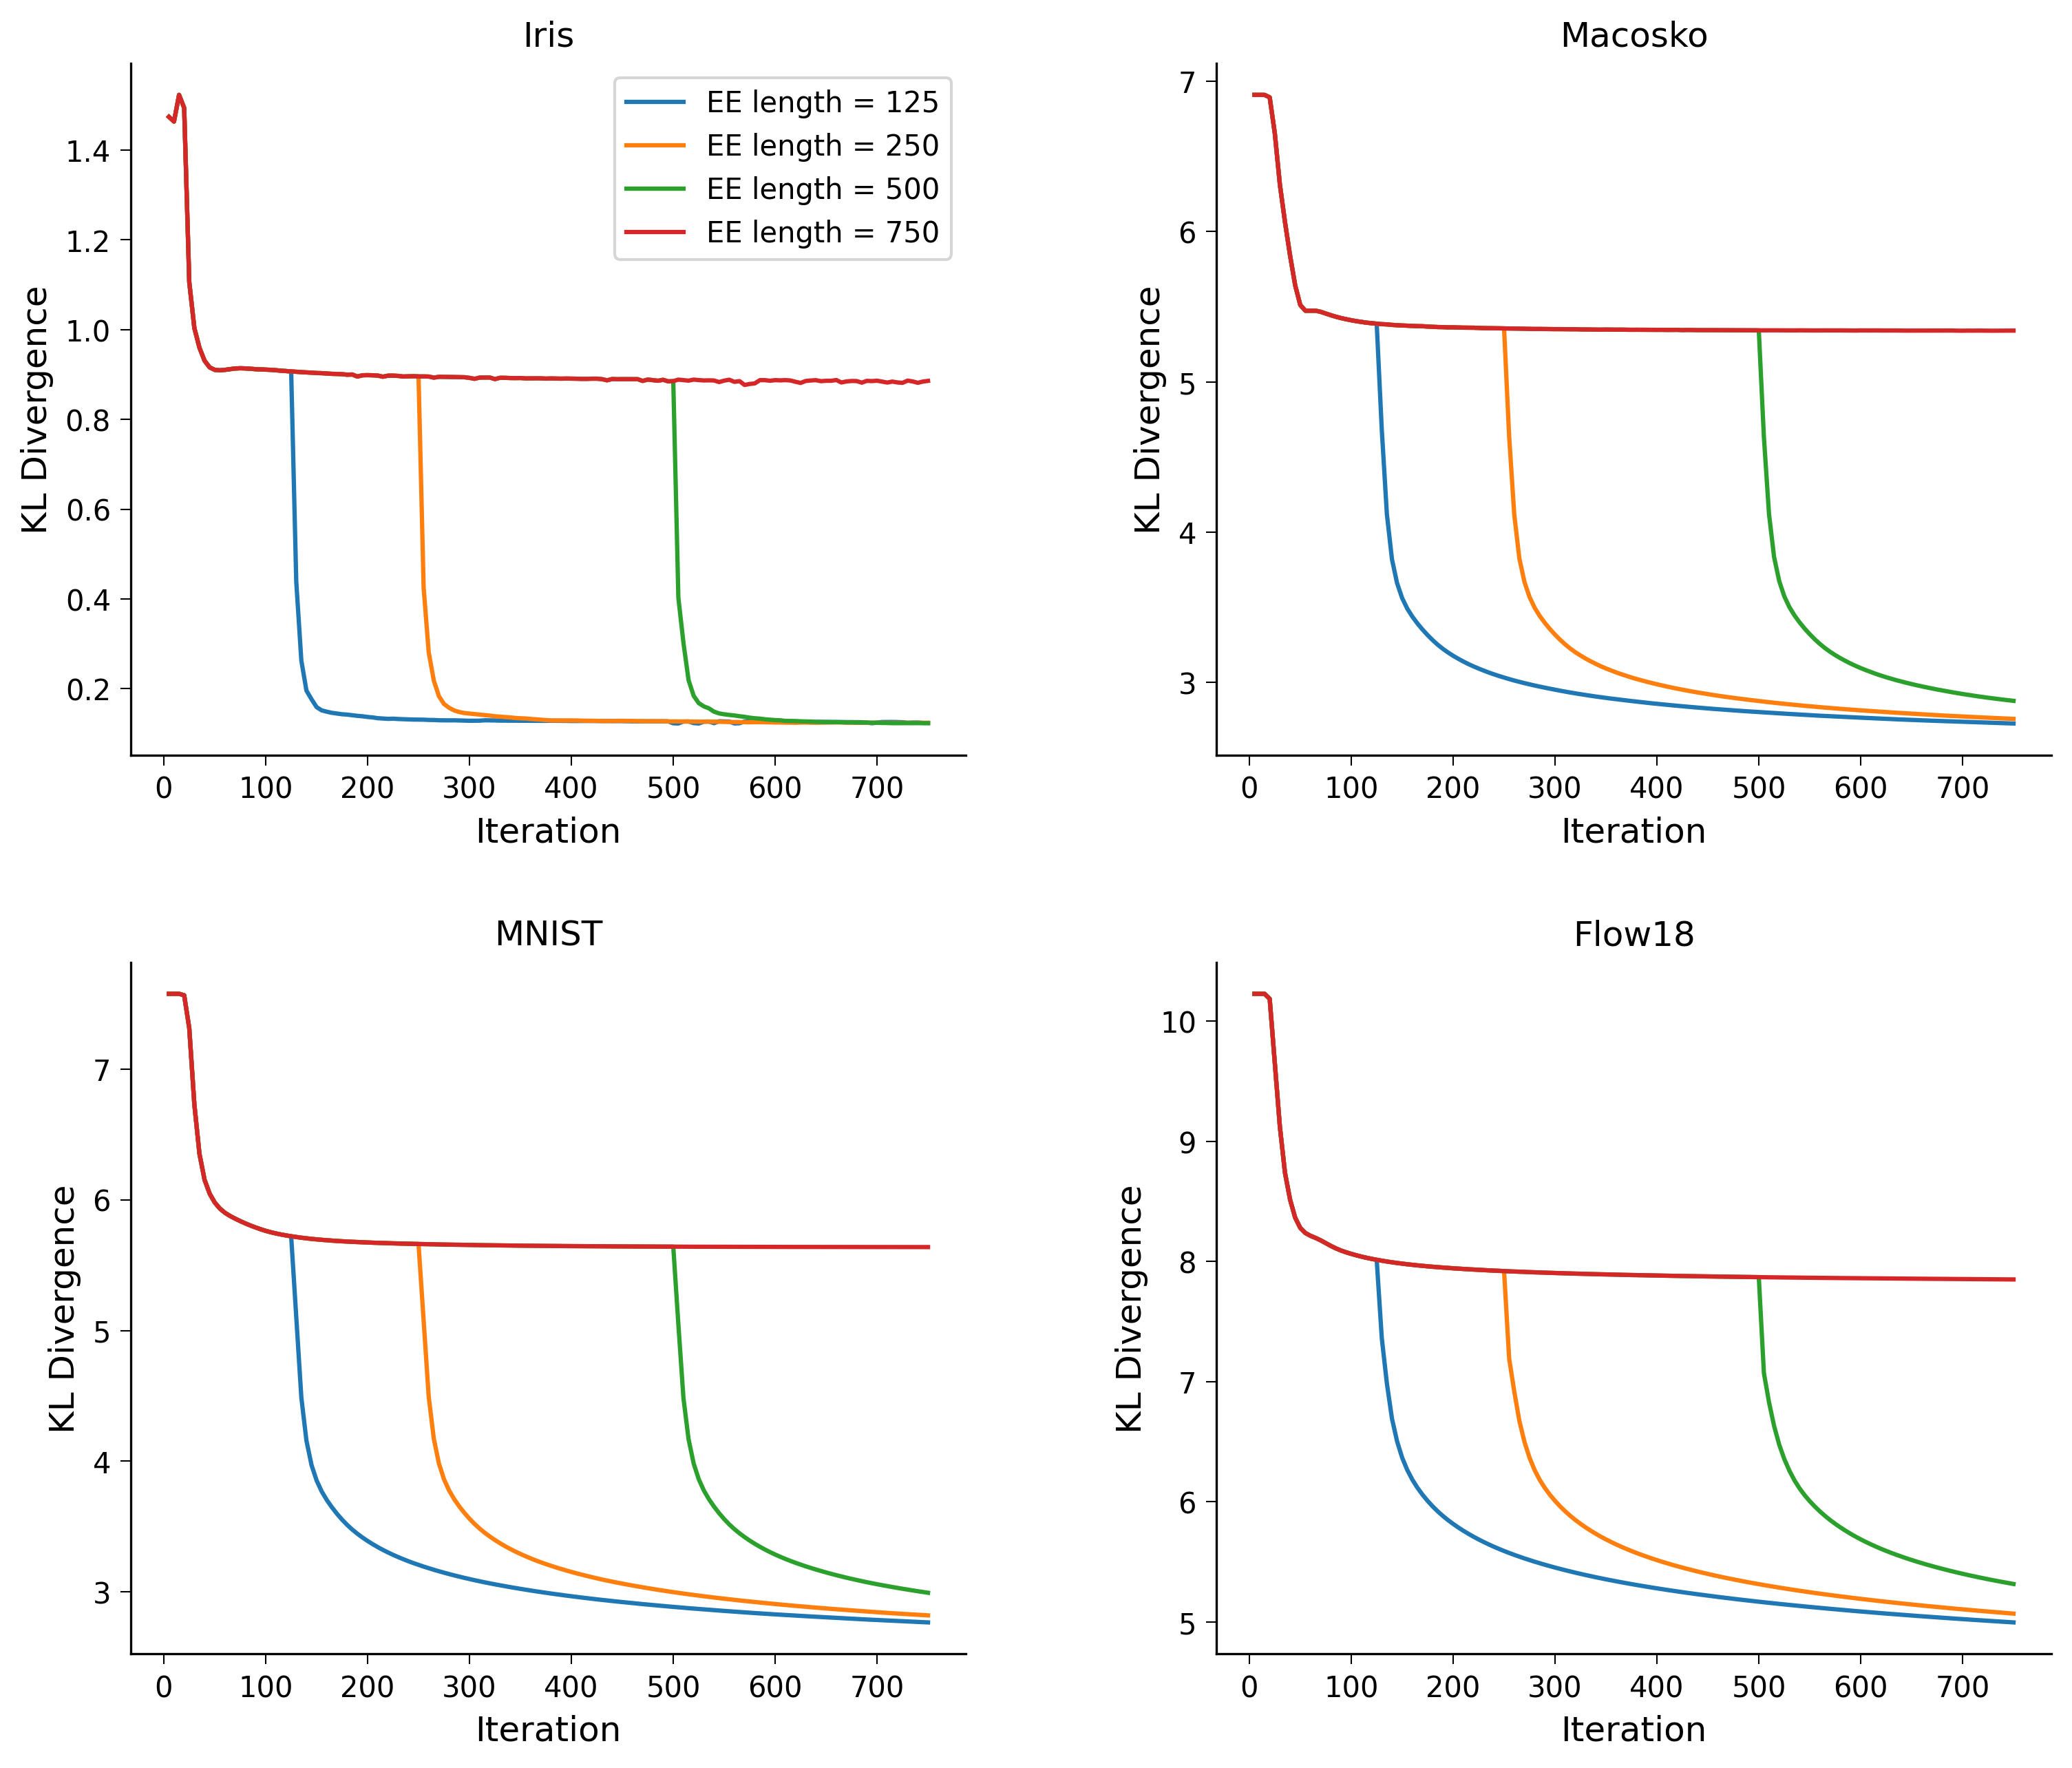
\includegraphics[width=\linewidth]{../code/figures/ee_length_kl_divergences_grid.png}
        \caption{t-SNE embeddings with different EE lengths - KLD.}
    \label{fig:EE_length_kld}
\end{figure}

\begin{figure}[h]
    \centering 
        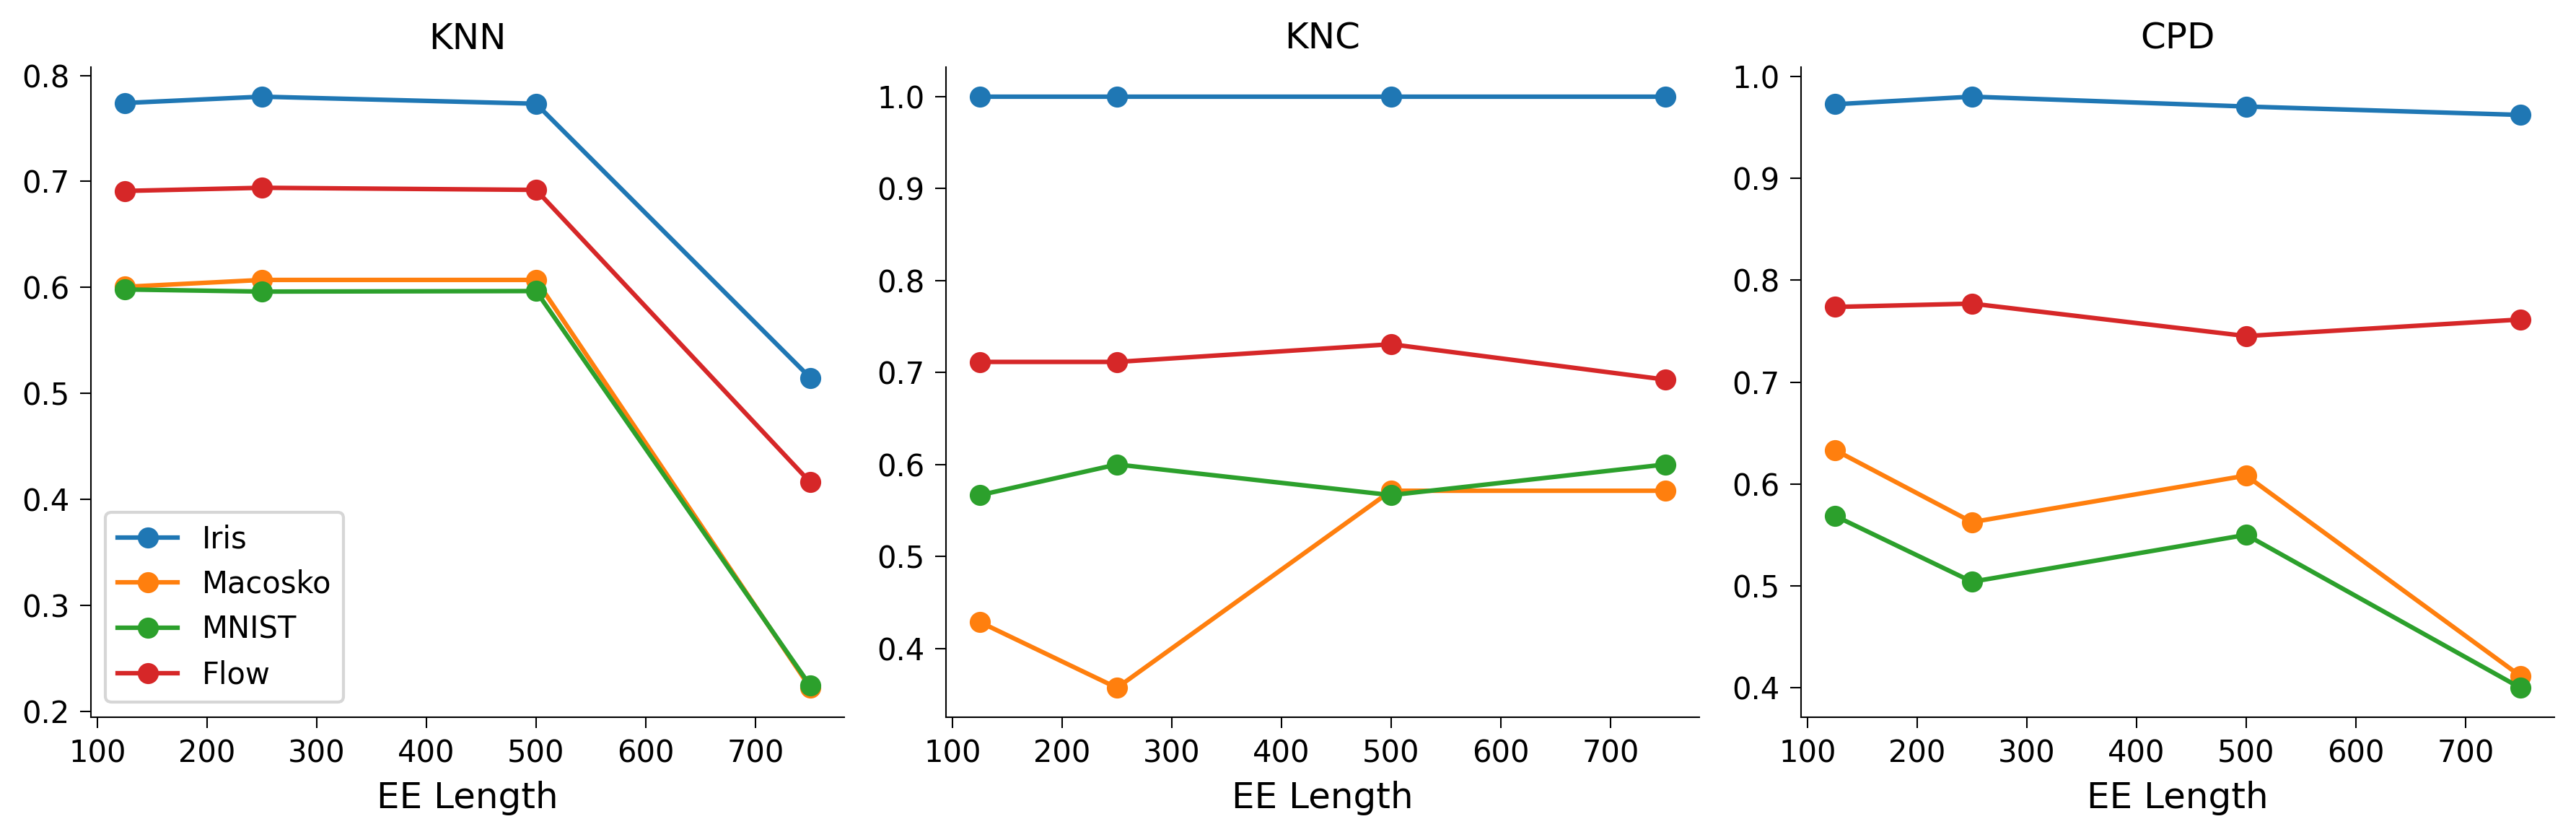
\includegraphics[width=\linewidth]{../code/figures/ee_length_3_quality_measures.png}
        \caption{t-SNE embeddings with different EE lengths - quality measures}
    \label{fig:EE_length_quality}
\end{figure}


\newpage 
\section{opt-SNE Implementation}
\comment{TODO: add description of what I did / what settings were used exactly}

\begin{figure}[h]
    \centering 
        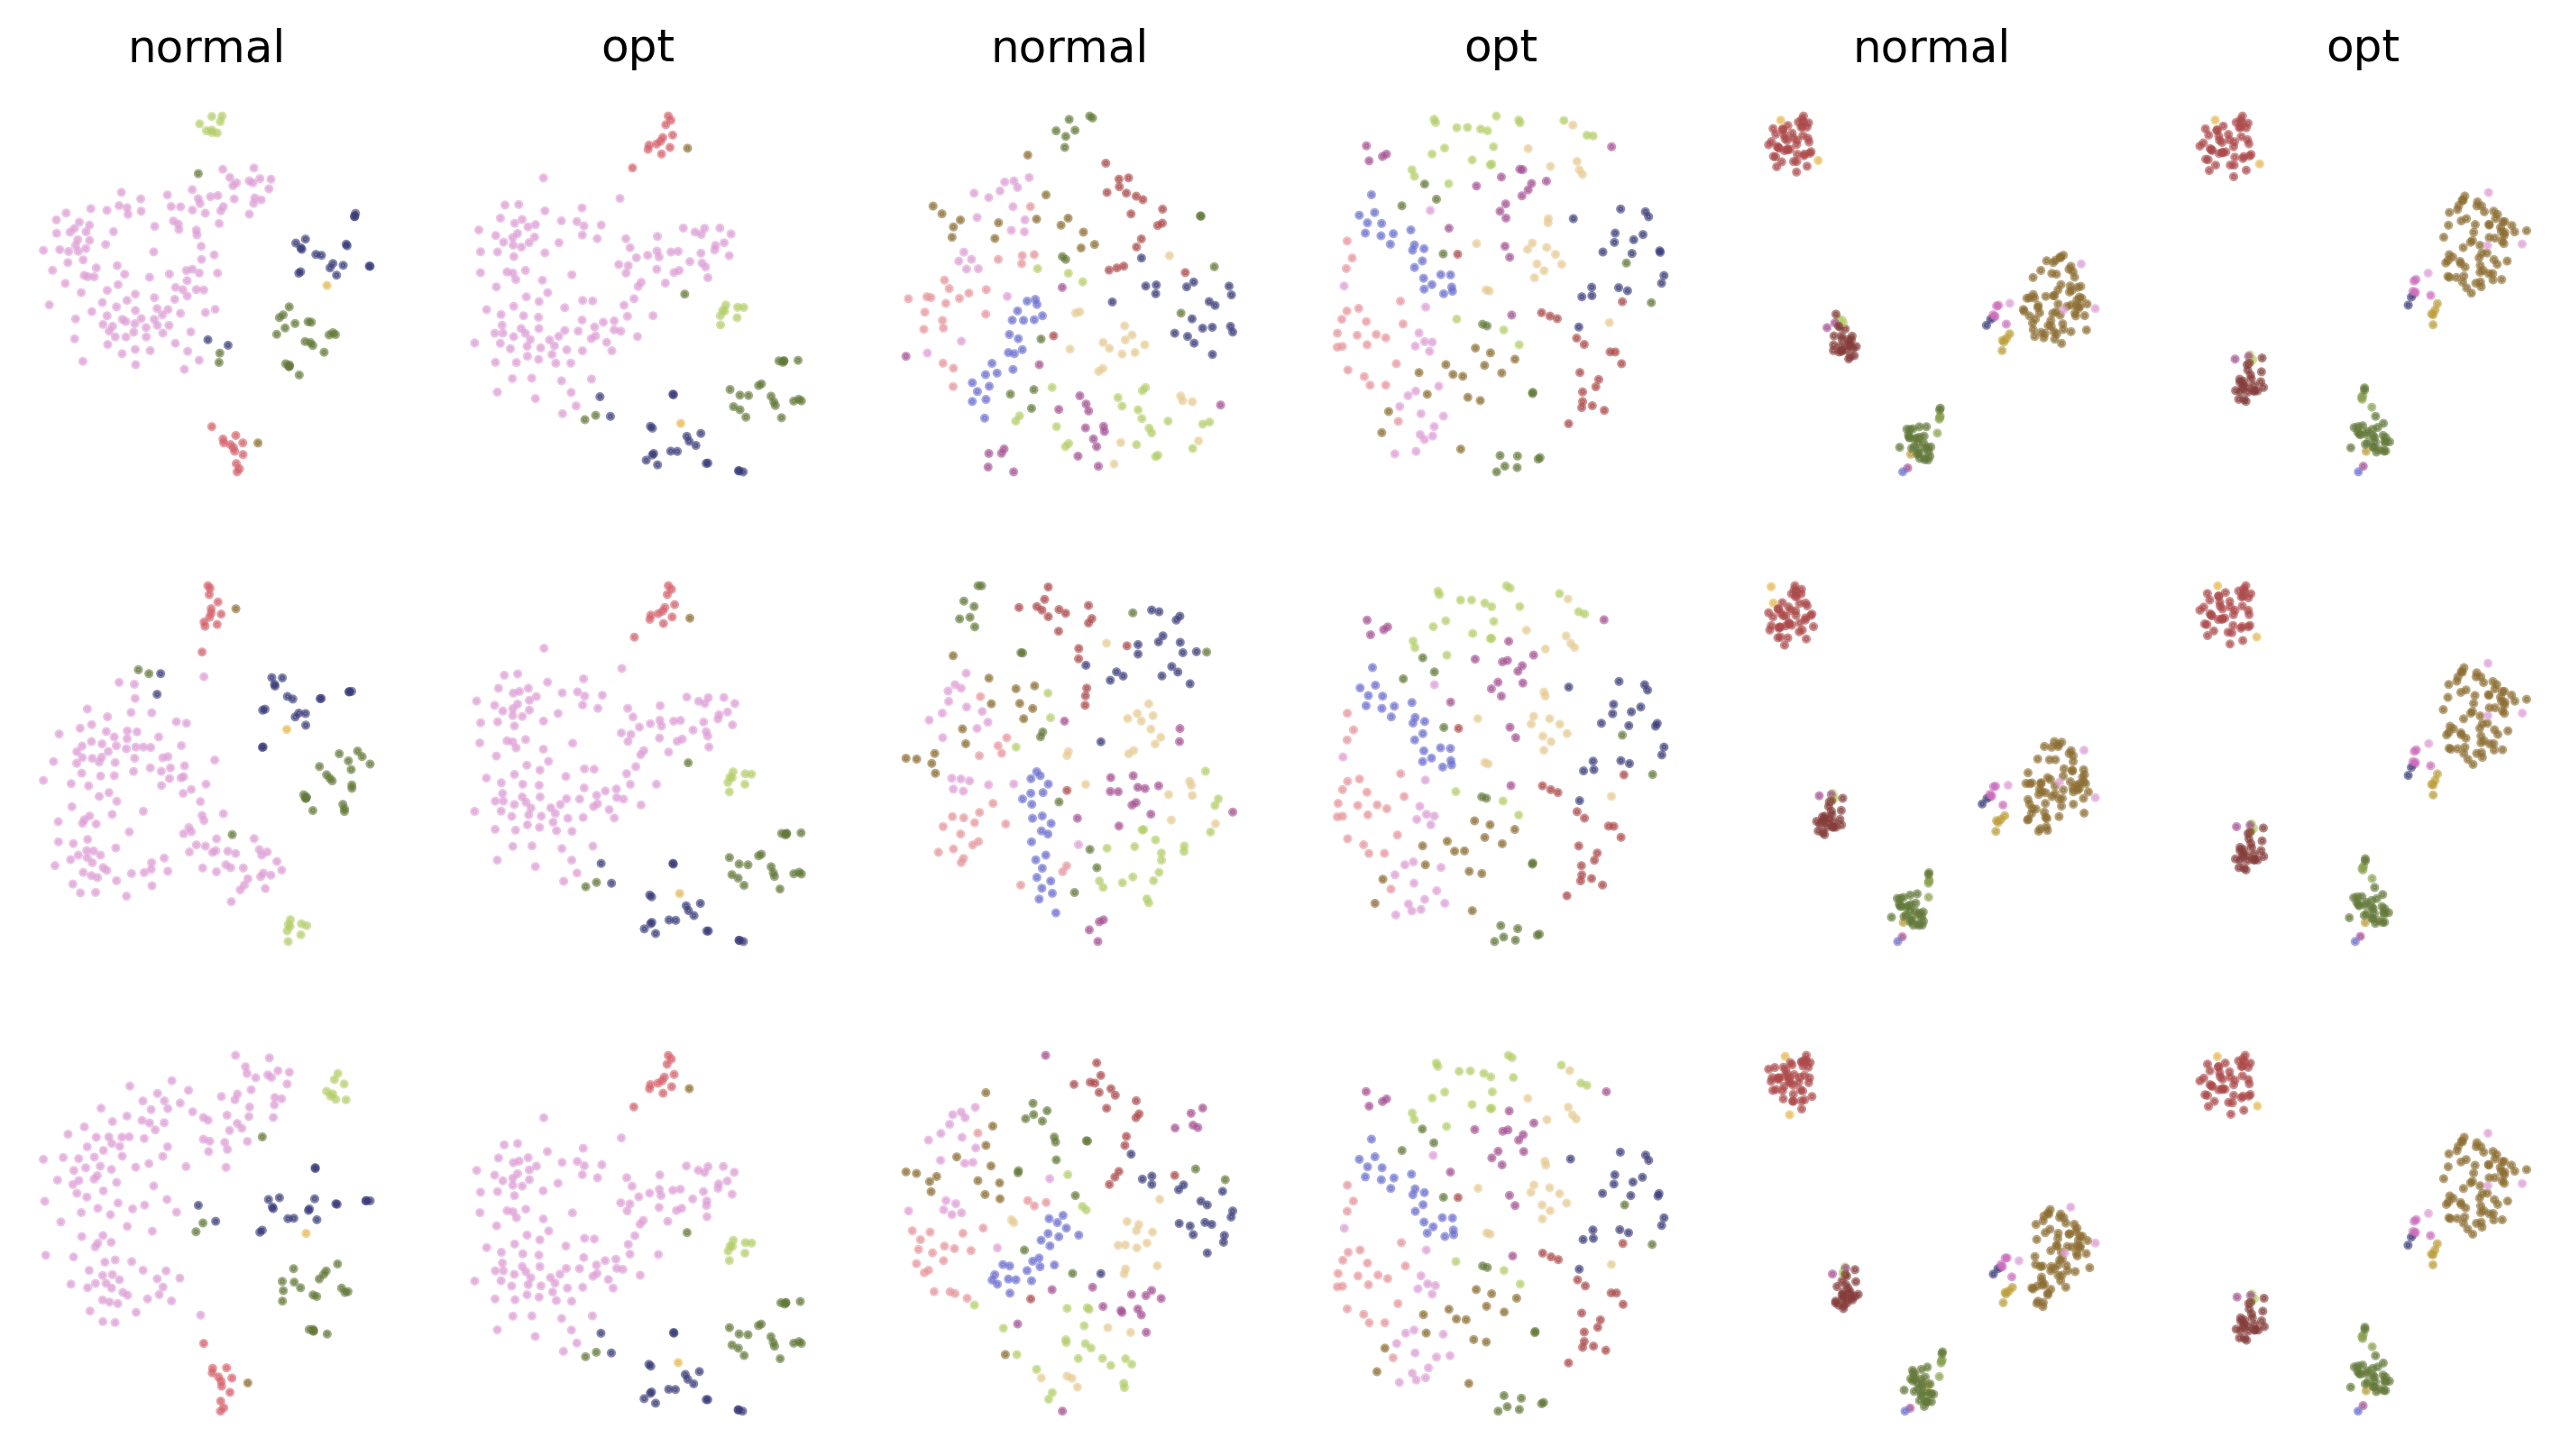
\includegraphics[width=\linewidth]{../code/figures/opt-SNE_embedding_grid_tab20b.png}
        \caption{t-SNE embeddings with and without automated stopping.}
    \label{fig:opt-SNE_grid}
\end{figure}

\begin{figure}[h]
    \centering 
        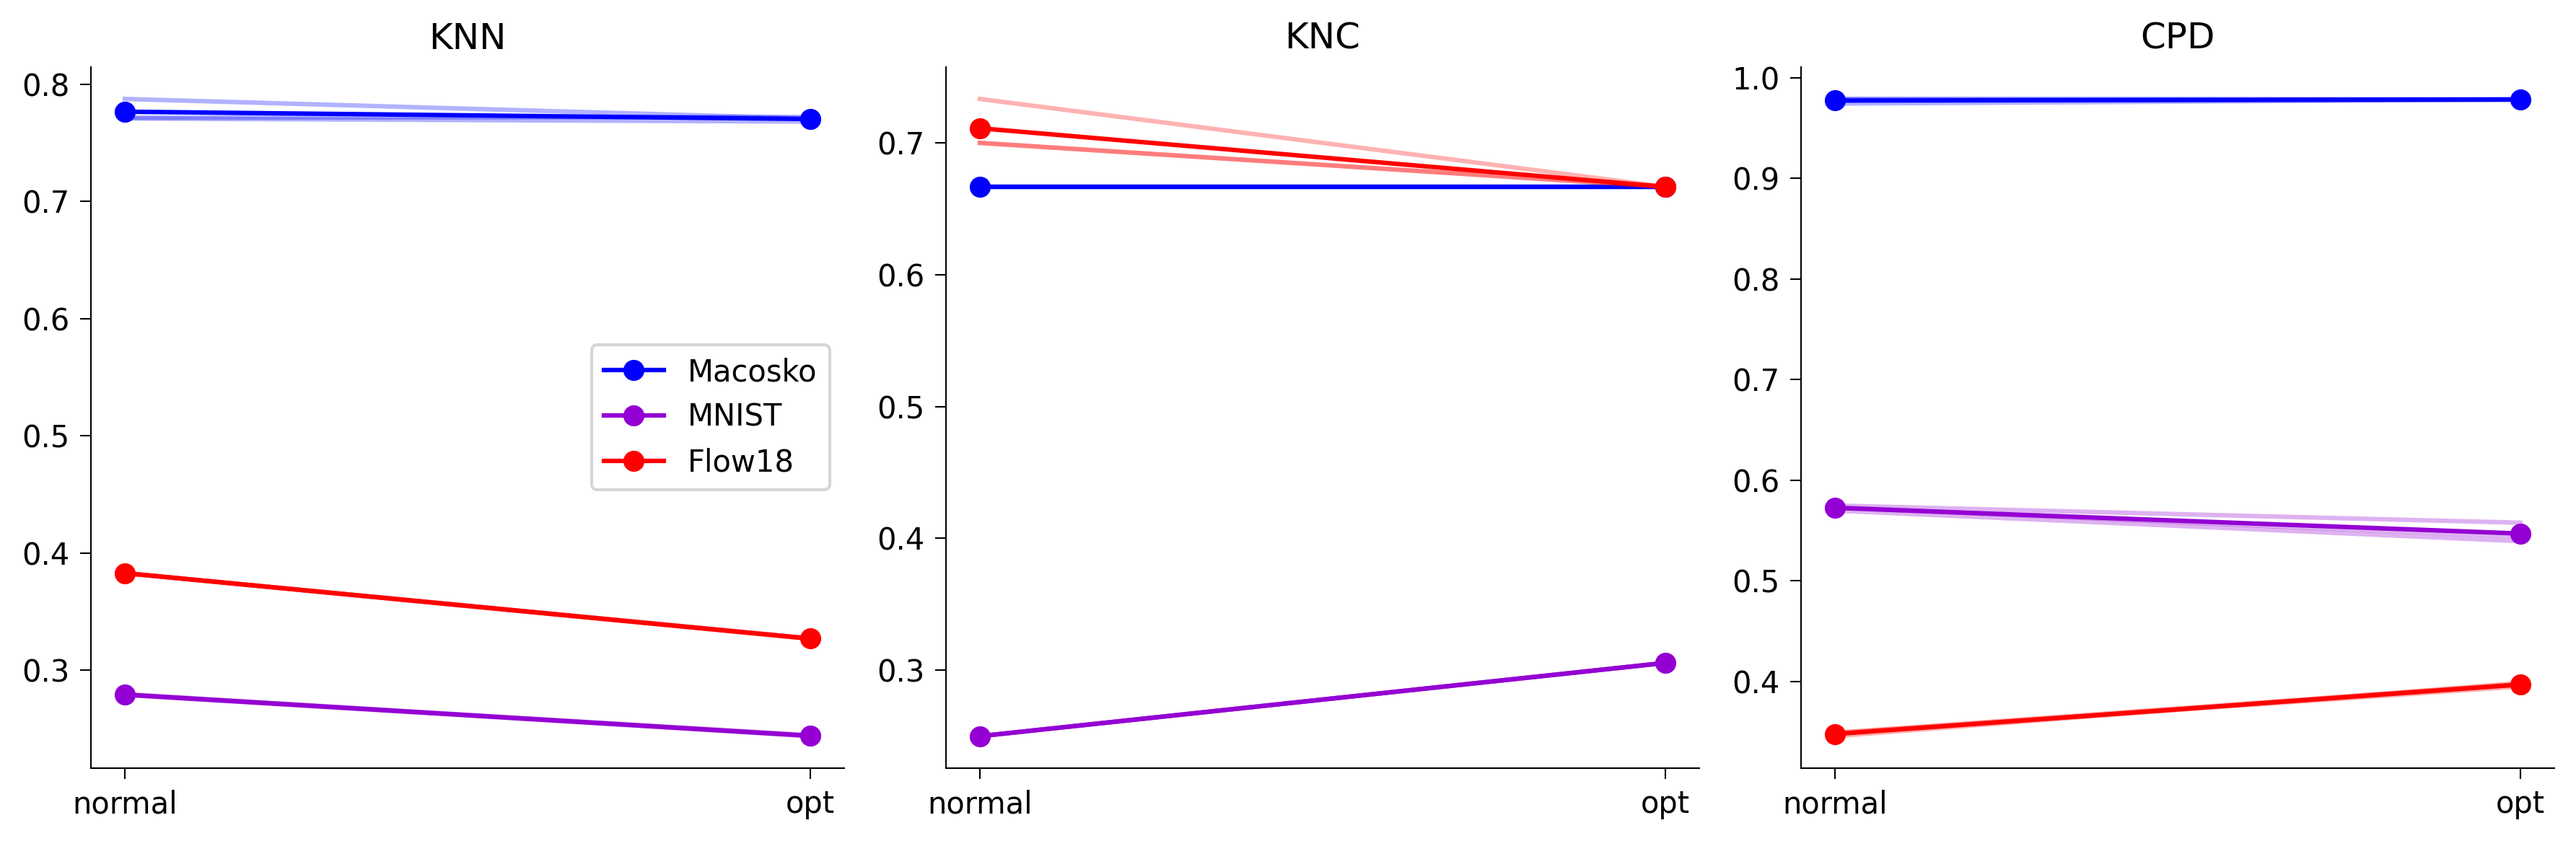
\includegraphics[width=\linewidth]{../code/figures/opt-SNE_3_quality_measures.png}
        \caption{Quality of t-SNE embeddings with and without automated stopping.}
    \label{fig:opt-SNE_quality}
\end{figure}

\begin{figure}[h]
    \centering 
        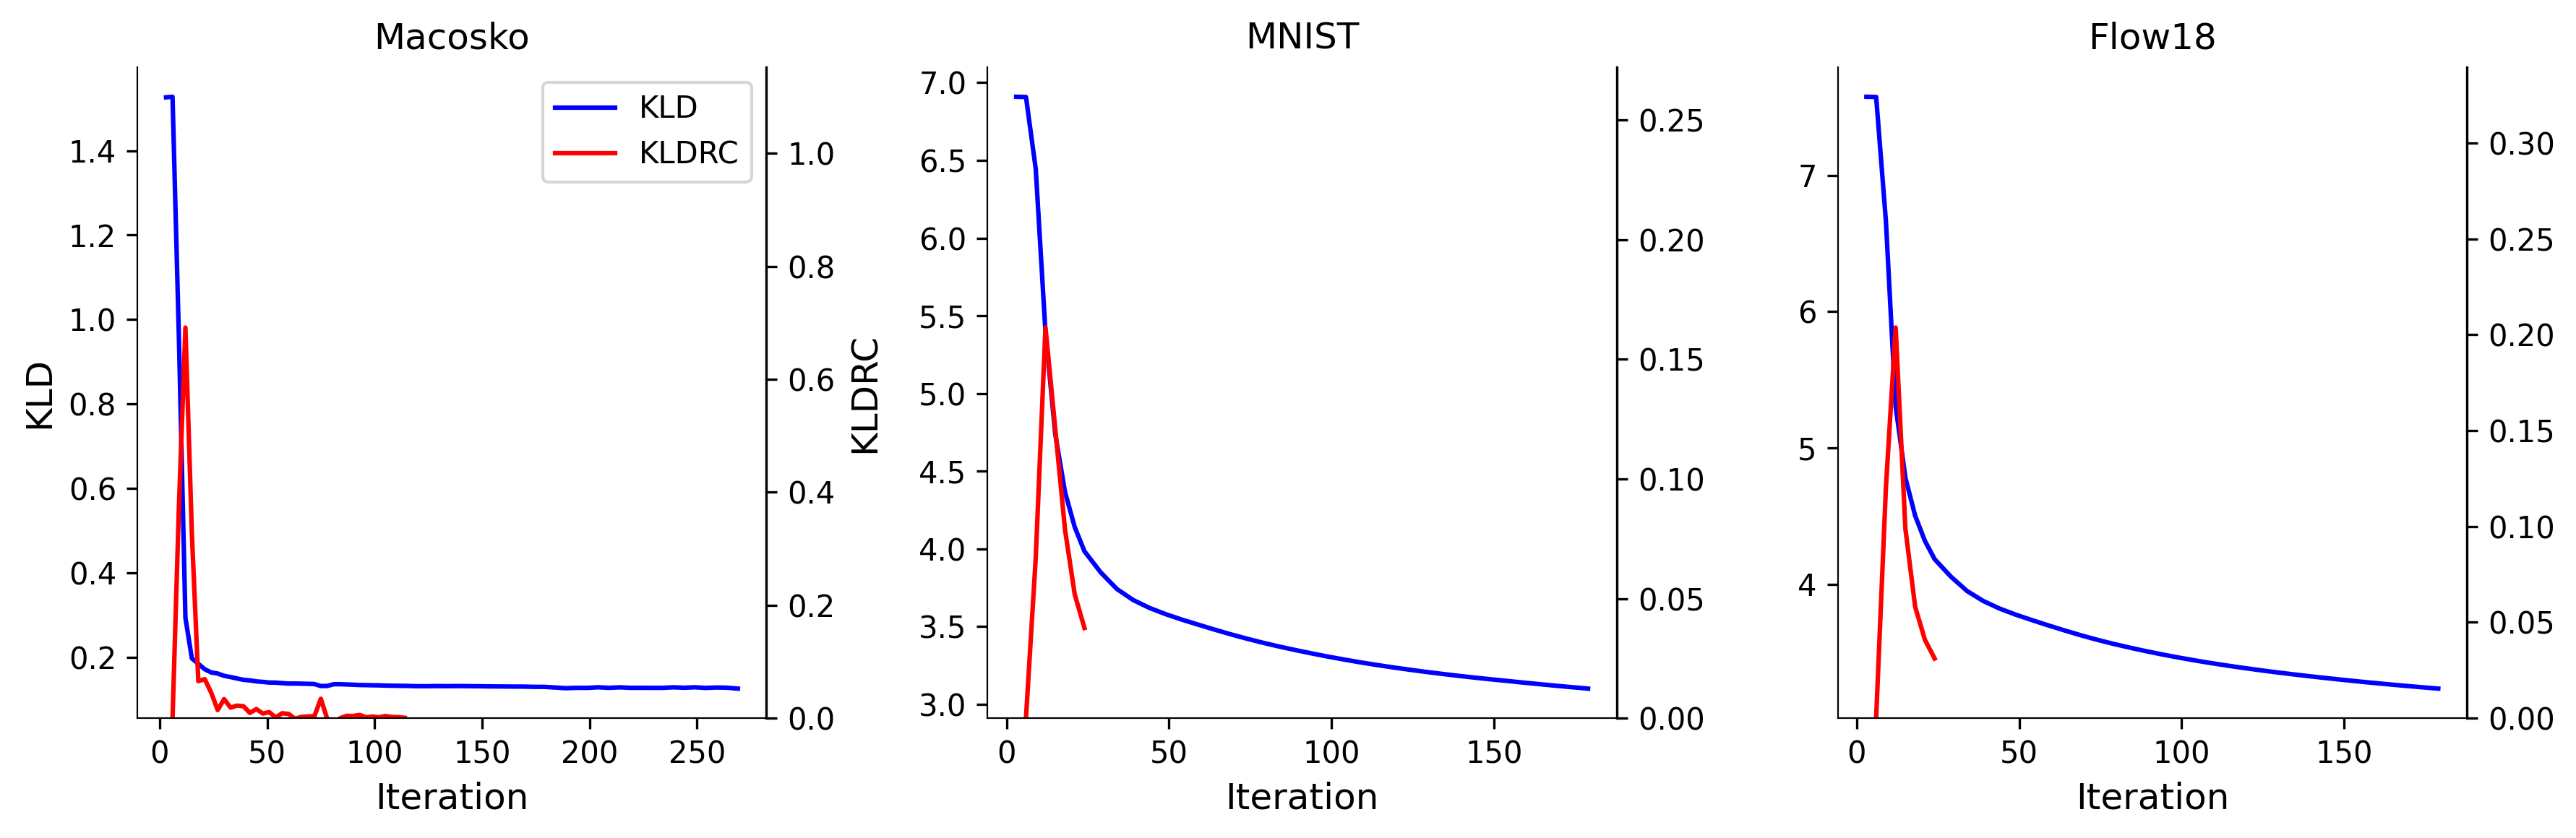
\includegraphics[width=\linewidth]{../code/figures/opt-SNE_kl_divergences_plot.png}
        \caption{KLD of t-SNE embeddings with and without automated stopping.}
    \label{fig:opt-SNE_kld}
\end{figure}